\documentclass{sig-alternate-10pt}

\usepackage{epsfig,xspace,multirow,capt-of,comment}
\usepackage[hyphens]{url}
\usepackage{hyperref}
\usepackage[hyphenbreaks]{breakurl}
\usepackage{graphicx,amssymb,amsmath,endnotes}
\usepackage{times}
\usepackage{subfigure}
\usepackage{ulem}
\usepackage{rotating}
\usepackage{wasysym, pifont}
\usepackage[usenames,dvipsnames]{color}
\usepackage{placeins}
\usepackage{balance}
\usepackage{epstopdf}
\epstopdfsetup{update}
%%%%%
% used in QxDM section
\usepackage{algorithmic}
\usepackage{algorithm}
\usepackage{array}
\usepackage{tabularx}
\usepackage{enumitem}
%%%%%
% for subfigure and space adjustment
%\usepackage[demo]{graphicx}
%\usepackage{subcaption}
%\usepackage[showframe]{geometry}
%\usepackage{amsthm}
%\theoremstyle{definition} \newtheorem{apitest}{Test}

\setcounter{secnumdepth}{5}

\hyphenpenalty=7000
\tolerance=600

\normalem

\newcommand{\rot}[1]{\begin{sideways}#1\end{sideways}}
%\newcommand{\mysection}[1]{\vspace{-.00in}\section{#1}\vspace{-.00in}}
%\newcommand{\mysubsection}[1]{\vspace{-.00in}\subsection{#1}\vspace{-.00in}}
%\newcommand{\mysubsubsection}[1]{\vspace{-.00in}\subsubsection{#1}\vspace{-.00in}}

\newcommand{\MR}[1]{\multirow{2}{*}{#1}}

\newcommand{\mysection}[1]{\vspace{-.07in}\section{#1}\vspace{-.02in}}
\newcommand{\mysubsection}[1]{\vspace{-.05in}\subsection{#1}\vspace{-.02in}}
\newcommand{\mysubsubsection}[1]{\vspace{-.05in}\subsubsection{#1}\vspace{-.02in}}


\newcommand{\hd}[1]{\small{\textbf{\texttt{#1}}}\normalsize}
\newcommand{\hds}[1]{\small{\textbf{\texttt{#1}}}}
\newcommand{\hdf}[1]{\small{\textbf{\texttt{#1}}}\footnotesize}

\newcommand{\ISP}{$\sf\small{ISP}$}
\newcommand{\ISPP}{$\sf\small{ISP}$ }
\newcommand{\UMICH}{$\sf\small{UMICH}$}
\newcommand{\UMICHH}{$\sf\small{UMICH}$ }

\newcommand{\YY}{\CIRCLE}
\newcommand{\NN}{\Circle}
\newcommand{\YN}{\RIGHTcircle}
\newcommand{\XX}{\ding{53}}

\newcommand{\Ignore}[1]{{\small }}
\newcommand{\mycomment}[1]{{\color{red}[\textsf{#1}]}}



\specialcomment{Notes}{%
        \noindent$\bf\Rightarrow\Rightarrow$%
}{%
        $\Leftarrow\Leftarrow$%
}
\providecommand{\Note}[1]{%
        \noindent{\bf$\Rightarrow\Rightarrow$#1$\Leftarrow\Leftarrow$}%
}
\newcommand{\Donothing}{\ignorespaces\ifhmode\unskip\fi}
\newcommand{\HideNotes}{%
        \excludecomment{Notes}%
        \renewcommand{\Note}[1]{\Donothing}%
}

%here is how to use it:
%\TReport{ test}
%\begin{TReports}
%test 
%\end{TReports}

\specialcomment{TReports}{%
}{%
}
\providecommand{\TReport}[1]{%
        \noindent{#1}%
}
\providecommand{\Paperonly}[1]{%
        \noindent{#1}%
}

\newcommand{\HideTReport}{%
        \excludecomment{TReports}%
        \renewcommand{\TReport}[1]{\Donothing}%
}

\newcommand{\HidePaperOnly}{%
        \renewcommand{\Paperonly}[1]{\Donothing}%
}

\definecolor{gray}{rgb}{0.5,0.5,0.5}
\newcommand{\etc}{\emph{etc.}\xspace}
\newcommand{\ie}{\emph{i.e.,}\xspace}
\newcommand{\eg}{\emph{e.g.,}\xspace}
\newcommand{\etal}{\emph{et al.}\xspace}
\newcommand{\wrt}{\emph{w.r.t.}\xspace}
\newcommand{\aka}{\emph{a.k.a.}\xspace}
\newcommand{\AlgBox}[1]{{\framebox[1.2\width]{\textbf{#1}}}}

\renewcommand{\paragraph}[1]{\smallskip\noindent{\bf{#1.}}}
\newcommand{\paragrapha}[1]{\smallskip\noindent{\bf{#1}}}
%\renewcommand{\algorithmiccomment}[1]{//#1}

\makeatletter
  \newcommand\figcaption{\def\@captype{figure}\caption}
  \newcommand\tabcaption{\def\@captype{table}\caption}
\makeatother

\newcommand{\vsp}{\vspace{+0.15in}}

\newcommand{\nsection}[1]{\vspace{-1em}\section{#1}\vspace{-0.7em}}
\newcommand{\nsubsection}[1]{\vspace{-0.85em}\subsection{#1}\vspace{-0.55em}}
\newcommand{\nsubsubsection}[1]{\vspace{-0.4em}\subsubsection{#1}\vspace{-0.3em}}
\newcommand{\ncaption}[1]{
 	\vspace{-1.5em}
	\caption{#1}
 	\vspace{-1.3em} % sometime two figure might overlap because of this
}

%\HideTReport
\HidePaperOnly

\begin{document}
%\title{Discovering RRC State Behavior and Performance Implications in Cellular Networks}
\title{Discovering RRC Transient States, Behavior and Performance Implications in Cellular Networks}

% TODO figure out authors:  order and who at Tmobile do we include?

%\dagger is more pretty
\author{
Sanae Rosen$^\#$, Haokun Luo$^\#$, Z.~Morley Mao$^\#$, Jie Hui$^*$, 
Aaron Drake$^*$, Kevin Lau$^*$\\
$^\#$University of Michigan, $^*$T-Mobile USA Inc.\footnotemark
} % end author

\iffalse
\numberofauthors{6}
\author{
\alignauthor
Sanae Rosen \\
	\affaddr{University of Michigan} \\
%	\affaddr{Ann Arbor, MI} \\
%	\email{\normalsize sanae@umich.edu} \\
\alignauthor
Haokun Luo \\
	\affaddr{University of Michigan} \\
%	\affaddr{Ann Arbor, MI} \\
%	\email{\normalsize haokun@umich.edu} \\
\alignauthor
Z. Morley Mao \\
        \affaddr{University of Michigan} \\
%        \affaddr{Ann Arbor, MI} \\
%	\email{\normalsize zmao@umich.edu} \\
\and
\alignauthor
Jie Hui \\
        \affaddr{T-mobile} \\
%        \affaddr{Seattle, WA} \\
%        \email{\normalsize Jie.Hui@t-mobile.com} \\
\alignauthor
Aaron Drake \\
        \affaddr{T-mobile} \\
%        \affaddr{Seattle, WA} \\
%        \email{\normalsize Aaron.Drake@t-mobile.com} \\
\alignauthor
Kevin Lau \\
        \affaddr{T-mobile} \\
%        \affaddr{Seattle, WA} \\
%        \email{\normalsize Kevin.Lau@t-mobile.com} \\
}
\fi

%\large{Paper ID: 75 \hspace{0.5in} Number of Pages: 10+1}

\maketitle


\footnotetext{The views presented here are as individuals and do not necessarily reflect any position of T-Mobile.} 

% ABSTRACT

Slow network experience on smartphone could hurt user experience and downgrade application reputation. When users are urgent about specific information, the carried information size is small but the latency of the mobile network service is very sensitive. The discontinuous burst of short data transmission is the most common traffic pattern in the cellular network. But significant latency appears at the beginning part of the data transmission. In order to identify the root cause, I use diagnostic cross layer monitoring tool, QxDM (Qualcomm eXtensible Diagnostic Monitor), and found that inactive response to packet loss in the RLC (Radio Link Resource) leads to unnecessary timeout in the transport layer. I propose a RLC \textit{Fast Re-Tx (Retransmission)} mechanism to avoid sluggish reaction to packet loss, and further reduce the latency during the initial network connection. Based on our simulation results, the \textit{Fast Re-Tx} mechanism could reduce the latency by up to \textit{35.69\%} over initial network connection.


\section{Introduction}
%\renewcommand{\labelitemii}{$\star$}
Cellular network technologies, such as 3G \textit{Universal Mobile Telecommunications System} (UMTS) and 4G \textit{Long Term Evolution} (LTE), require that devices transition between various RRC states based on the network traffic patterns of individual mobile clients.  These states have different performance and energy consumption tradeoffs, as well as different state transition delays.  Using high-power RRC states only when necessary allows users to experience good network performance on resource-constrained mobile devices. Although the RRC states are defined by \textit{3rd Generation Partnership Project} (3GPP)~\cite{spec-3G-RRC, spec-LTE-RRC}, many aspects of the RRC state machine, such as timers for transitioning between states, are implementation or configuration-specific, differing by device model, network operator and location.  The real-world deployment of RRC state machines and the impact on performance are not well-understood. 

A better understanding of RRC state behavior would be beneficial for many parties.  Cellular network operators would be interested in determining how devices on their networks perform and how performance can be improved.  Device manufacturers would be interested in detecting device-dependent effects --- device implementation details and features such as Fast Dormancy~\cite{fast_dormancy} can mean different devices perform differently. Developers of major applications might be interested in understanding how network behavior can impact application performance, as work has been done to show that application behavior can decrease RRC-related performance issues~\cite{aro}.  Finally, researchers studying protocol optimization would find a better understanding of RRC state behavior valuable. 

In this paper, we examine how RRC states are implemented, behave and perform in real-world implementations. We present a new approach to inferring RRC state transitions that addresses limitations in previous work which prevent inference from being done in non-ideal network conditions or by non-expert users. In particular, we focus on detecting performance anomalies caused by RLC-layer \textit{transient states}, which can have a significant performance impact. We perform a study of RRC state implementations and performance on 16 network operators from 9 countries,  and use RLC layer analysis to understand the root causes of behavior and performance trends discovered. We present three main categories of contributions: %. First, we present several methodological contributions which allow us to perform measurements that lead to a deeper understanding of RRC behavior. Second, we present our findings on previously unknown performance problems and phenomena. Third, we suggest some potential performance optimizations. 

%\begin{enumerate}[noitemsep,topsep=0pt,parsep=0pt,partopsep=0pt]
%[noitemsep,topsep=0pt,parsep=0pt,partopsep=0pt]
%\item
\noindent\labelitemi\indent \textbf{Methodological contributions.} We have created two types of tools. First, we designed a novel generic RRC state model inference method that is robust to poor network conditions and interfering background traffic on the mobile device. It is implemented in an Android application and is designed to be usable out of the box by non expert users.  We focus primarily on inferring the demotion timers of RRC states as well as the performance associated with each state. We hope to release this tool as open-source software. Second, we determined methods to effectively make use of RLC-layer traces from \textit{Qualcomm eXtensible Diagnostic Monitor} (QxDM). We developed a novel cross-layer mapping mechanism that correlates transport layer packets with data layer link \textit{protocol data units} (PDUs, the smallest data transmission unit in RLC). It can successfully map 99.8\% of transport-layer packets to PDUs. This allows the root causes of TCP and UDP performance and packet loss issues to be accurately identified at the RLC layer.

%\item
\noindent\labelitemi\indent  \textbf{New Findings on the Impact of RRC State on Performance.} We analyze the RRC state implementation and associated performance characteristics for a number of network operators, showing that our methods are useful in understanding RRC states in the real world. We present several new findings that show there are significant undetected performance problems in networks today. At the RLC layer, we show that there are frequent RLC-layer retransmission delays surrounding \textit{transient states}, especially during state transitions to and from FACH. 

%\item 
\noindent\labelitemi\indent \textbf{Proposed Solution to Performance Problems Found.} We propose an improvement to how RLC currently behaves based on our improved understanding of RLC-level behavior. To reduce potentially unnecessary retransmissions that occur during poorly-performing FACH-related transient states, we propose an RLC \emph{Fast Re-Tx} mechanism that actively responds to the RLC PDU loss signals. By simulating this fast retransmission mechanism using real QxDM traces that provide visibility of RLC traffic behavior, we find that our proposed mechanism could reduce RLC latency by up to 35.69\% when these poorly-performing FACH states occur. In other states, the latency is still reduced by 2.66\% on average.

% The possible latency overhead occurs when we fail to speculate the RLC retransmission, but the overall latency could still be reduced by 2.66\%.
%\end{enumerate}


%%	\begin{itemize}
%		\item
%			\textbf{Methodology:} Based on state of art RRC state inference method, we designed a generic RRC state model generation mechanism to effectively reduce the effect of unstable wireless channel, and produce finer RRC state machine using classic statistical method. In additional, we develop the first cross layer mapping mechanism in the empirical study to correlate the transport layer packets with the data layer link PDUs, so that we could accurately identify the TCP/UDP performance issue inside the RLC layer. We could map 99.8\% of the transport layer packets to the corresponding RLC layer PDUs.
%		\item
%			\textbf{Observation:} We observe the abnormal large FACH state latency issue through our RRC inference measurement. After a world wide scale deployment of RRC state model generation measurement, we are able to discover the device dependent and network specific abnormal FACH state behaviors. We also observe the frequent RLC layer retransmission and retransmission delay over initial FACH state and FACH promotion transition, which contributes a lot to the transport layer latency.
%		\item	
%			\textbf{Implications:} Due the abnormal initial FACH state and FACH latency behavior, the application could batch the data transmission to reduce the possible number of transmission over FACH. To address the RLC retransmission delay issue, we propose a RLC \emph{Fast Re-Tx} mechanism to active response to the RLC PDU loss signals. By simulate the fast retransmission mechanism in the real trace QxDM, we apply cost-benefit analysis and found that \emph{Fast Re-Tx} could reduce RLC latency up to 35.69\% over FACH states.
%	\end{itemize}

\section{Background}\label{sec:background}

\begin{figure}[t!]
\centering
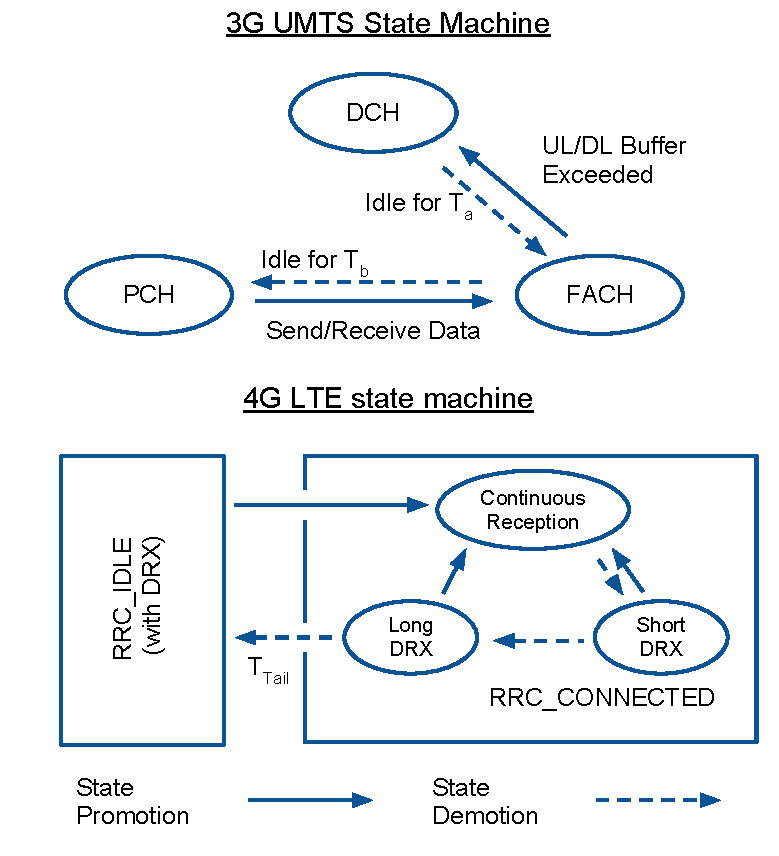
\includegraphics[width=0.5\textwidth]{figs/RRC_State_Diagram.pdf}
\ncaption{Possible 3G and 4G State Machines as Specified by 3GPP.} 
\label{fig:statemachine}
%\begin{center}
%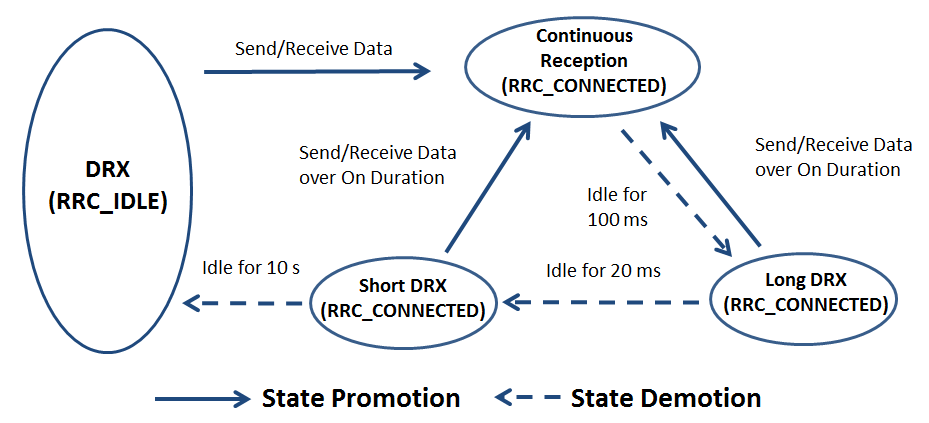
\includegraphics[width=0.5\textwidth]{figs/4g_rrc.png}
%\end{center}
%\ncaption{4G LTE state machine based on our inference methodology}
%\label{fig:4G_statemachine}
\vspace{0.5em}
\end{figure}

\begin{figure}[t!]
\centering
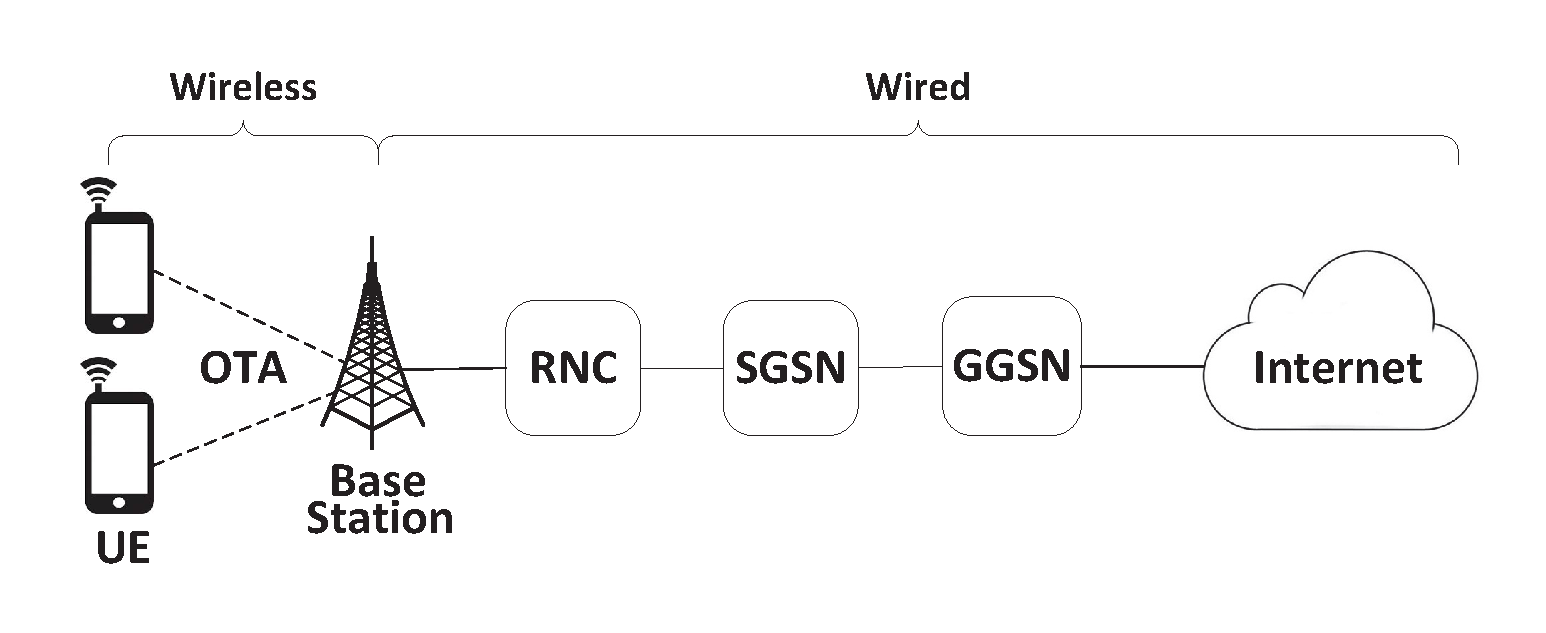
\includegraphics[width=0.5\textwidth]{figs/cellular_network_topology.eps}
\ncaption{The general cellular network architecture}
\label{fig:cell.topology}
\end{figure}

As illustrated in Figure~\ref{fig:cell.topology}, in both 3G UMTS~\cite{3gpp.3G} and 4G LTE networks~\cite{3gpp.lte}, data is transmitted from \textit{user equipment} (UE), i.e. mobile devices,  to the base station (Node B in UMTS, eNB in LTE), then to the \textit{Serving GPRS support node} (SGSN) and \textit{Gateway GPRS support node} (GGSN), and ultimately to the server~\cite{umts_book}. The link between the UE and the base station is known as the \textit{over-the-air} (OTA) link, and it is the only wireless link in the network topology. The rest of the links from the base station to the internet are all wired.

Mobile cellular networks use the Radio Resource Control (RRC) protocol to allocate resources to mobile devices.  Handsets transition between different RRC states, which vary in power consumption and bandwidth, and an individual RRC state machine is maintained for each handset.  Transitions between different states occur due to traffic patterns between the device and base station. In general, more traffic will cause a higher-power and higher-bandwidth state to be entered.  The RRC protocol for these network types has been defined by 3GPP~\cite{spec-3G-RRC, spec-LTE-RRC}.

Different carriers implement RRC state machines differently, with state transitions and different associated timers varying between carriers.  However, for 2G, 3G and 4G LTE, there are a fixed set of possible states defined. We give a brief overview below; a more detailed overview can be found in previous work~\cite{3g_rrc, 4g_rrc}.

\begin{table*}[th!]\small
\begin{tabularx}{\textwidth}{ | c | c | X | }
\hline
\textbf{Category} & \textbf{Label} & \textbf{Description} \\
\hline
\hline
%\multicolumn{2}{|c|}{\textbf{3G UMTS - Specification}} \\
%\hline
%\multirow{3}{*}{\textbf{\vbox{3G UMTS - Specification}}} & DCH & high-power, high-bandwidth\\ \cline{2-3}
\multirow{3}{*}{\textbf{3G UMTS - RRC States in Specification}} & DCH & High-power, high-bandwidth\\ \cline{2-3}
& FACH & Low-power, low-bandwidth\\ \cline{2-3}
& PCH & No transmission possible\\
\hline
%\multicolumn{2}{|c|}{\textbf{3G UMTS - Observed Phenomena}} \\
%\hline
%\multirow{7}{*}{\textbf{\vbox{3G UMTS - Observed Phenomena}}} & FACH TRANSITION & period of high latency when transitioning from DCH to FACH\\ \cline{2-3}
\multirow{5}{*}{\textbf{3G UMTS - Newly-detected Transient States}}
& FACH INIT & Initial FACH state interval with \textit{frequent} link layer retransmission\\ \cline{2-3}
& FACH PROMOTE & State transition interval from FACH to DCH with signalling overhead\\ \cline{2-3}
& FACH STABLE & Time interval in between FACH INIT and FACH PROMOTE\\ \cline{2-3}
& PCH INIT & Initial PCH state interval with \textit{few} link layer retransmission\\ \cline{2-3}
& PCH PROMOTE & State transition interval from PCH to FACH with signalling overhead\\ \cline{2-3}

\hline
\multirow{1}{*}{\textbf{3G UMTS - UDP-Layer Observed Behavior}} & FACH TRANSITION & Period of high latency when transitioning from DCH to FACH\\
\hline
\hline
%\multicolumn{2}{|c|}{\textbf{4G LTE - Specification}} \\
%\hline
%\multirow{2}{*}{\textbf{\vbox{4G LTE - Specification}}} & RRC CONNECTED & high-power, high-bandwidth \\ \cline{2-3}
\multirow{2}{*}{\textbf{4G LTE - RRC States in Specification}} & RRC CONNECTED & High-power, high-bandwidth \\ \cline{2-3}
& RRC IDLE & No transmission possible \\
\hline
%\multicolumn{2}{|c|}{\textbf{4G LTE - Observed Phenomena}} \\
\hline
%\multirow{1}{*}{\textbf{\vbox{4G LTE - Observed Phenomena}}} & FACH TRANSITION & period of high latency when transitioning from DCH to FACH \\
\multirow{1}{*}{\textbf{4G LTE - UDP-Layer Observed Behavior}} & LTE TRANSITION & Period of high latency when demoting from RRC CONNECTED to RRC IDLE\\
\hline
\hline
%\multicolumn{2}{|c|}{\textbf{QxDM Related}} \\ 
%\hline
\multirow{3}{*}{\textbf{QxDM Related}} & RLC retx ratio & $\frac{\textit{\# of Retx PDUs in \textbf{T}}}{\textit{Total \# of PDUs in \textbf{T}}}$ , where \textit{\textbf{T}} is a range of time \\ \cline{2-3}
& UDP loss ratio & $\frac{\textit{\# of UDP packets \textbf{NOT} received by receiver in \textbf{T}}}{\textit{Total \# of UDP packets that the sender transmitted in \textbf{T}}}$ , where \textit{\textbf{T}} is a range of time \\ \cline{2-3}
& Inter-packet interval & Time between when a test packet is sent and when a high-power state is induced, for the purpose of measuring timers. \\ \cline{2-3}
\hline
\end{tabularx}
\ncaption{Summary of key terminology used.} % Terminology should not be plural, a terminology is a set of terms and we have only one set of terms. https://en.wiktionary.org/wiki/terminology
\label{tab:terminology}
\end{table*}

For 3G UMTS~\cite{spec-3G-RRC}, there are three main states:  DCH, which is high-power and high-bandwidth, FACH, which is low power and low bandwidth, and PCH, where no transmission is possible. If a higher-bandwidth state is needed, there is a promotion delay. Some carriers may always go directly from PCH to DCH. An example RRC state machine can be seen at the top of Figure~\ref{fig:statemachine}. These terms are summarized in Table~\ref{tab:terminology}.
%As a further complication, UMTS supports \emph{fast dormancy}. The user device is able to proactively request to transition to IDLE to reduce the tail time after a data transmission where the device is a higher-power state than necessary~\cite{fast_dormancy, spec-3G-RRC}.

For 4G~\cite{spec-LTE-RRC}, the state machine is more complicated, and is summarized in the bottom half of Figure~\ref{fig:statemachine}.  We are concerned mainly with transitions between RRC\_{}CONNECTED, a higher-power state, and RRC\_{}IDLE, a lower-power state where no data is transmitted. The other states have timers on the orders of tens or hundreds of milliseconds are are not practical to measure on end-user devices, as tools such as a power monitor are required.

%There are two main states: RRC\_{}CONNECTED, a higher-power state, and RRC\_{}IDLE, a lower-power state.  RRC\_{}IDLE periodically wakes up to determine if it needs to promote to a higher-power state.  This is known as Discontinuous Reception or DRX.  We would like to infer the timer to fall back to RRC\_{}IDLE, as well as the time between ON segments in RRC\_IDLE and the length of those segments.

%For RRC\_CONNECTED, there are several additional substates.  After a data transfer, the device remains in Continuous Reception for some time, before transitioning to Short DRX.  Similarly to DRC for RRC\_IDLE, the device sleeps for a short period of time, waking up periodically to check if there is data, but the sleep time is much shorter.  There is another timer to transition to Long DRX, which has a longer sleep timer than Short DRX, but still a much shorter one than in RRC\_IDLE. Additionally, the ON timers for the three DRX states can vary~\cite{spec-LTE-RRC}.

Determining when to fall back to a low power state can have a substantial impact on performance, as can the state transitions supported.  If demotion happens early, then there will be additional promotion delays, resulting in decreased user performance.  If it happens late, then an unnecessary amount of power will be consumed. For this reason, we wish to understand how carriers implement RRC state machines in practice.

Furthermore, we found that network traffic often does not follow the ideal pattern expected by the RRC specification, another major motivation for understanding RRC state behavior in the real world.  This occurs in particular during state transitions, where certain transitions on certain devices can lead to substantial delays, so we define terms to refer to these phenomena which we will use throughout the paper. There is often a significant additional promotion delay immediately after a state demotion, especially a demotion from DCH to FACH.  We refer to this phenomenon as \emph{FACH\_{}TRANSITION} when it occurs immediately before FACH, and \emph{LTE\_{}TRANSITION} when it occurs in LTE. 

To understand the root cause of this unexpected behavior, we observed behavior at the RLC layer.  We break down the behavior in each state at the RLC layer into several smaller \emph{transient states} as shown in Figure~\ref{fig:qxdm.rrc.state}.  

% XXX I rewrote this paragraph.
We define the FACH\_{}PROMOTE and PCH\_{}PROMOTE transient states based on behavior observed at the RRC layer. These states end when the new RRC state is logged by QxDM and start when the previous IP data packet was sent.  We describe the experiments to determine when this period occurs in~\ref{sec:exp.setup}.  The FACH\_{}INIT transient state corresponds to a period of high RLC retransmissions determined experimentally from the QxDM traces.  The period of FACH not covered by FACH\_{}PROMOTE and FACH\_{}INIT we define to be FACH\_{}STABLE.  There is no corresponding PCH\_{}STABLE state as no data is sent in PCH.  Therefore, the PCH\_{}INIT transient state refers to the period of time in PCH during our tests where the device is not in PCH\_{}PROMOTE.  We determined that the FACH\_{}TRANSITION delays occur primarily due to losses in the transition states FACH\_{}INIT and FACH\_{}PROMOTE.

%Both the FACH\_{}PROMOTE and PCH\_{}PROMOTE transition states are determined by the average time interval between the last IP data packet log timestamp to the next RRC state log timestamp from the local QxDM experiments that will be defined in ~\ref{sec:exp.setup}. The FACH\_{}INIT substate is where the high RLC retransmission occurs. We determine the average time interval value where the substantial high RLC retransmission from those QxDM experiments as well. We exclude the whole FACH state period by the FACH\_{}PROMOTE and FACH\_{}INIT to get FACH\_{}STABLE substate. The PCH\_{}STABLE substate doesn't exist since the device cannot stay in PCH during the PCH to FACH promotion. So we determine the PCH\_{}INIT substate period by subtracting PCH\_{}PROMOTE substate interval from the PCH state interval.

\begin{figure}[t!]
\centering
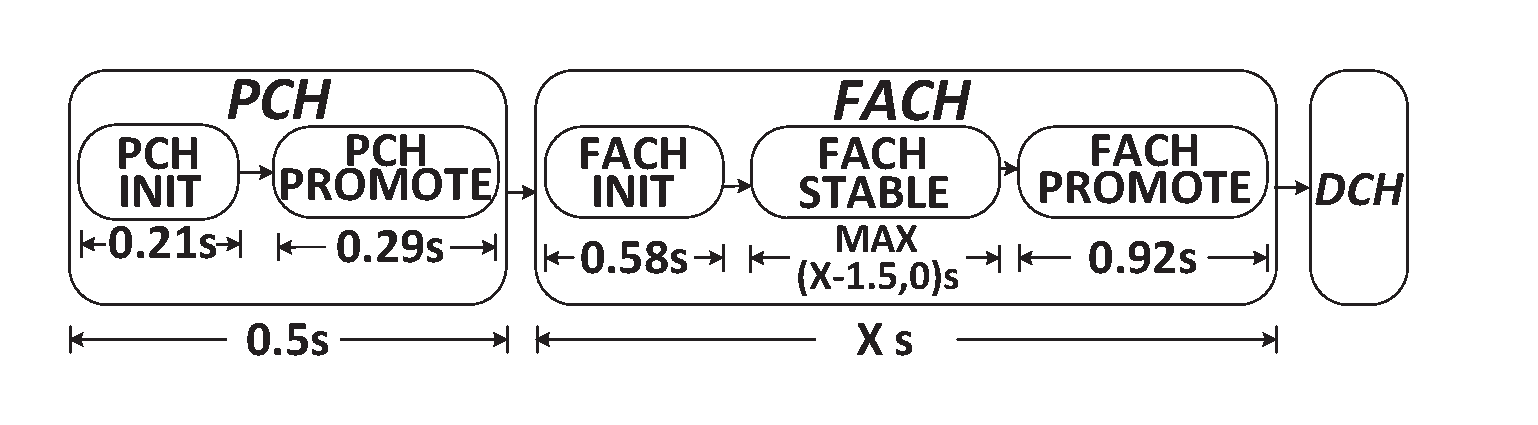
\includegraphics[width=0.5\textwidth]{figs/qxdm_rrc_state_no_pch_stable.eps}
\vspace{-2.5ex}
\ncaption{RRC transient state definitions from observed RLC-layer behavior during state promotions. We examine these individually through QxDM to investigate root causes of latency.} 
\label{fig:qxdm.rrc.state}
\vspace{-1.5ex}
\end{figure}

%We call the period of time immediately after a promotion from DCH to FACH \emph{FACH\_{}INIT}, and the period of time where FACH promotes to DCH \emph{FACH\_{}PROMOTE}.  FACH\_{}TRANSITION occurs where FACH\_{}INIT is immediately followed by FACH\_{}PROMOTE; FACH\_{}TRANSITION refers to a type of behavior observed at the UDP layer and not to RLC-level behavior.  Similarily, PCH is divided into \emph{PCH\_{}INIT} and \emph{PCH\_{}DEMOTE}.

%\mycomment{these terminology on INIT, PROMOTE, and DEMOTE are not quite clear, maybe explain in terms of signaling required:  Does INIT mean that there are still signaling occurring?}

\section{RRC State Inference\\Methodology}\label{sec:methodology}

The 3GPP specifications leave some implementation details, such as specific timers, to the carriers~\cite{spec-LTE-RRC,spec-3G-RRC}. It has been shown in previous work~\cite{3g_rrc} that it is possible to infer RRC state transition timers using differences in RTT values for different inter-packet timings.  As transitions between states involve overhead, it is possible to infer the RRC state at a given time by sending a packet to deliberately trigger a promotion to a higher state and measuring the resulting RTT.  By varying the spacings between packets it is possible to determine demotion timers, and by varying packet sizes it is possible to detect promotions triggered by large data transmissions.

A large-scale survey of the RRC state machines of different carriers would be valuable in understanding how RRC state machines are implemented by carriers and perform in practice.  Additionally, it would allow us to determine if, for a specific carrier, there are differences between phone models or geographic regions.  It is possible that carriers may make use of different equipment vendors in different markets, leading to RRC implementation differences.  Also, some aspects of RRC behavior are known to be device-dependent, such as fast dormancy~\cite{fast_dormancy}. RRC transitions involve both the device and base-station, so device-specific differences are possible, and in ~\S\ref{sec:clientresults} we discuss some which we have detected.

We have also found that the performance trends expected from the RRC state specification is not reflective of the performance clients experience in practice. A motivating example of the problem can be seen in Figure~\ref{fig:rtt_raw_data_22}.  22 sets of RRC state measurements can be seen in the top graph, including results for both large (1 KB) and empty UDP packets. For this test, DCH is induced by sending a large packet, then another packet is sent after a time interval --- this interval is shown on the X-axis. The two packet sizes allow us to observe FACH, which is characterized by low latencies for small packets and higher latencies for large ones, as a state transition only occurs after sufficient data is transmitted.

It is clear from Figure~\ref{fig:rtt_raw_data_22} that the DCH state demotion timer is 2.5 to 3 seconds long, and the FACH timer is an additional three seconds, after which there is a transition to PCH. DCH is characterized by low RTTs, as there is no promotion delay.  PCH has much higher RTTs, due to the promotion delay, and FACH has a lower RTT for small packets due to the promotion delay not being required.  The ideal pattern that would be expected based on the RRC specification can be seen in the bottom graph.

There are two main differences between the measured values and the ideal behavior.  First, transitions, especially to FACH, involve long and unexpected latencies, which we will show are due to delays in promotion-related RLC-layer transient states.  Second, the measurements are very noisy, especially in PCH.  As a result, inferring RRC states from a small number of tests is not reliably accurate, and data processing is often needed for accurate results.


%There are some other unexplained phenomena, however.  After 2.5s there is a peak in average RTTs for about a second, that gradually trails off. BEtween the FACH and PCH there is also a sudden jump in RTTs.  Furthermore, there is a significant difference between the behaviour of small and large packets in PCH.  These are not explainable by a simple RRC model, and these delays have the potential to be quite significant.  This graph illustrates clearly the importance of measuring device-specific phenomena to understand the performance impact of RRC state transitions in the real world.
Evidently, there are several significant challenges that need to be addressed to detect these types of non-ideal RRC state behavior.  First, substantial processing is needed to be able to eliminate network noise and correctly infer RRC timers --- the data shown in Figure~\ref{fig:rtt_raw_data_22} is in fact less noisy than average. Furthermore, even with controlled experiments the high degree of variance in our measurements often precludes the use of the algorithm presented in previous work~\cite{3g_rrc}.  Likely a large increase in network traffic in the past few years has lead to the increased presence of noise in our data.  It seems unlikely that, as cellular networks become more congested, inference will become easier, so a more robust RRC state inference methodology is critical

Second, due to the assumption that devices will closely fit a specific pattern of behavior, unexpected phenomena caused by lower-layer behavior, such as FACH\_{}TRANSITION,  would not be identified by an algorithm based on matching data to a known RRC state pattern only.  With existing approaches, these delays would be misclassified as noise or PCH and overlooked.  To detect these phenomena, a more general approach is needed.  An approach agnostic to RRC state also has the benefit that only one implementation is needed for different network technologies, making a public deployment more practical.  We inferred timers for nine different network technologies in our public deployment.

Finally, the existing inference algorithm cannot run as an application on the end-user devices of non-experts, as it requires  all network traffic (including background traffic not under the user's control) to be paused during these tests.  In order to make a public deployment possible, it is necessary to modify the algorithm to ensure that it is robust in the presence of background traffic, does not interfere with existing applications and does not require root access.

\begin{figure}[t!]
\begin{center}
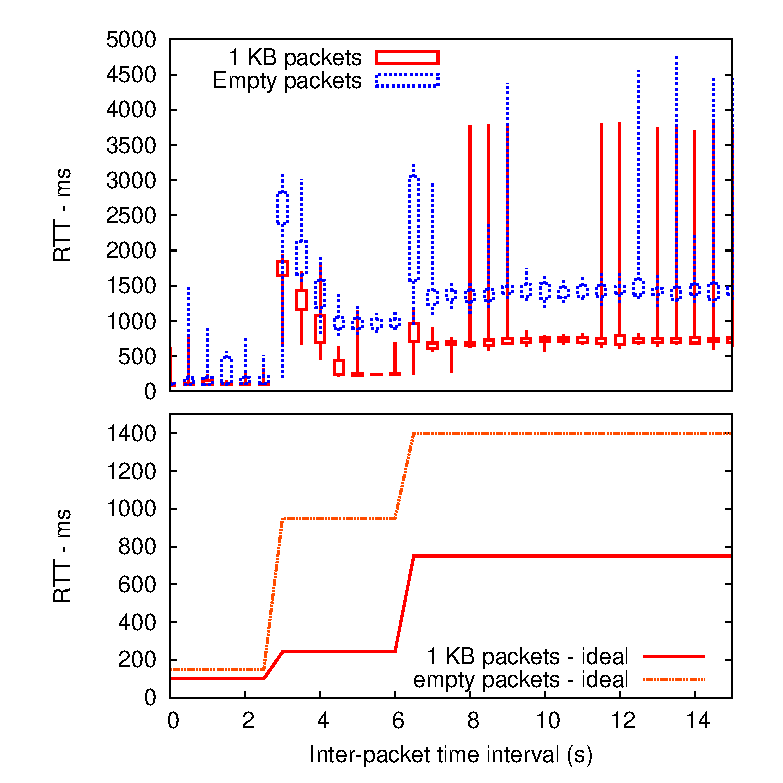
\includegraphics[width=0.45\textwidth]{figs/test_rrc_bad.eps}
\end{center}
\ncaption{Top graph: 22 measurements of RTTs as a function of time between packets. Ideally, we would expect it to appear like the lower, ideal graph, with no transmissions delays.}
\label{fig:rtt_raw_data_22}
\vspace{2ex}
\end{figure}

In developing these algorithms, we made use of three test devices, covering two models of phone and two carriers. \TReport{We examined T-Mobile and AT\&T, using one Samsung Galaxy SIII for each carrier as well as an HTC one on T-Mobile.}
We used QxDM to verify the ground truth for network timings for two of these devices, as well as to verify the presence of the anomalous FACH\_{}TRANSITION behavior and to determine the impact of RLC-layer transient states. We also validated our findings with a power monitor, as in previous work~\cite{3g_rrc, 4g_rrc}. Finally, in a controlled study with various devices on a single carrier\TReport{, T-Mobile,} using known RRC state machines (as described in \S\ref{sec:clientresults}) we verified that our inference algorithm is effective, including in higher-noise conditions. We also determined how much data is insufficient for the algorithm to work.  We compare our inferred timers with the QxDM-derived ground truth in \S\ref{sec:qxdm.analysis}.

We start by describing the client design below.

%Similar to the inference technique described in previous work~\cite{3g_rrc}, the core idea is to send a UDP packet that ensures the device starts in DCH state, then wait successively longer intervals before sending an additional UDP packet - either one large enough to always trigger a promotion to DCH, or a small one that can potentially be sent while remaining in FACH.  An echo server sends a packet back immediately so that the round-trip time of these two  packet types can be measured to deduce whether the device is in DCH, FACH or PCH.  A set of heuristics have been defined to identify which is which.

% TODO list heuristics before and after?

%First, as we have shown in our motivating example, it is not always entirely accurate to say that data falls into three clean, discrete and easy to identify states.  Even in IDLE or PCH, there can be significant differences between large and small packet RTTs (which makes our FACH heuristic a problem).  Furthermore, state transitions appear to often cause significant changes in RTTs - a number of ``pseudo-states" can appear, which can confuse a naive inference implementation. Just as importantly, it is this device- and carrier-specific anomalous behavior that we are trying to measure.

%Furthermore, this approach is tied to a specific network technology.  We do not want to have different algorithms for 3G, 2G and LTE if possible --- a general solution is much cleaner.  A generic state inference algorithm that can capture all of this anomalous behavior would be ideal.

%Additionally, we found that, while data that has been collected in the past is relatively noise-free, in practice the data collected can be very noisy, especially with weaker signal strengths.  This becomes particularly significant when trying to distinguish anomalous behavior during state transitions.  Is there a spike in RTTs due to delays on the network, or due to RTT-related delays?  If we have data from a small number of tests, this might not be obvious.  Even with many samples, it is valuable to be able to easily and efficiently determine the underlying RRC state patterns.

%Finally, in LTE specifically, many of the timers involved are very short, and very difficult to infer accurately due to the high level of noise in RTT measurements.  We investigate the feasibility of inferring these shorter timers, and show that, with the exception of those on the order of milliseconds, it is possible to infer these timers using packets to probe actively.  However, as there is significantly more overhead in detecting these fine-grained timers than in detecting timers on the order of seconds, we do not include this inference technique in our broader survey of RRC states.

\subsection{RRC Inference Client Design}
\begin{algorithm}[t!]\small
\begin{algorithmic}
\STATE {\textit{\textbf{Function} ClientDemotionTest():}}
\FOR{$n=0$ to $30$ inclusive} 
\FOR{$i=0$ to $9$} 
\STATE Send \emph{max} bytes, server echoes \emph{min} bytes.
\STATE Sleep $500n$ ms.
\STATE Send ten \emph{max} bytes, server echoes \emph{min} byte for each.
\STATE Record average RTT and packets lost (7s timeout).
\STATE Sleep $500n$ ms.
\STATE Send ten \emph{min} bytes, server echoes \emph{min} byte for each.
\STATE Record average RTT and packets lost (7s timeout).
\IF {No other traffic sent}
\STATE{record RTTs and losses}
\STATE{break from inner loop}
\ENDIF
\ENDFOR
\ENDFOR
\end{algorithmic}
\caption{Client-side data collection}
\label{alg:client_collection}
%\vspace{-0.5em}
\end{algorithm}

%\begin{TReport}
%\begin{algorithm}[t!]
%\begin{algorithmic}
%\STATE {\textit{\textbf{Function} FindDemotionModel:}}
%\FORALL{test runs from client}
%\STATE smoothData(smallPackets)
%\STATE smoothData(largePackets)
%\ENDFOR
%\FORALL{inter-packet time intervals}
%\STATE remove outliers and average across tests
%\ENDFOR
%\IF {Less than 10 complete tests}
%\STATE smooth all data again
%\ENDIF
%\STATE smallModel $\leftarrow$ Divide smallPackets into segments with similar RTTs
%\STATE largeModel $\leftarrow$ Divide largePackets into segments with similar RTTs
%\IF {time ranges of smallModel and largeModel inconsistent}
%\IF {differ by one data point}
%\STATE Pick segment range with smallest average error on measured data
%\STATE Re-calculate segment average values for the other model
%\ELSE
%\STATE Split larger mis-matched segment to align with other model
%\STATE Re-calculate segment average values for the  model
%\ENDIF
%\ENDIF
%\end{algorithmic}
%\ncaption{Server-side post-processing}
%\label{alg:client_collection}
%\end{algorithm}
%
%\begin{algorithm}[t!]
%\begin{algorithmic}
%\STATE {\textit{\textbf{Function} smoothData(data):}}
%\FOR{$i$ from $1$ to length(data) $-1$}
%\STATE d $\leftarrow \lvert data\lbrack i + 1 \rbrack - data\lbrack i - 1 \rbrack \lvert$
%\IF {$d < \frac{data\lbrack i - 1 \rbrack}{4}$}
%\STATE $newData\lbrack i \rbrack \leftarrow \frac{data\lbrack i + 1 \rbrack + data\lbrack i - 1 \rbrack}{2}$
%\ELSE 
%\STATE $newData\lbrack i \rbrack \leftarrow data\lbrack i \rbrack$
%\ENDIF
%\ENDFOR
%\RETURN newData
%\end{algorithmic}
%\ncaption{data smoothing algorithm used in server-side post-processing}
%\label{alg:client_collection}
%\end{algorithm}
%
%\begin{algorithm}
%\begin{algorithmic}
%\STATE {\textit{\textbf{Function} createPreliminaryModel(data, nCompleteTests):}}
%\STATE currentSegment $\leftarrow \lbrack \rbrack$
%\IF {more than 10 complete tests}
%\STATE $r1 \leftarrow 0.25$; $r2 \leftarrow 0.5$; $r3 \leftarrow 0.75$
%\STATE $in_spike \leftarrow 1$; $min_normal \leftarrow 2$
%\ELSE
%\STATE $r1 \leftarrow 0.5$; $r2 \leftarrow 0.75$; $r3 \leftarrow 1$
%\STATE $min_{spike} \leftarrow 2$; $min_normal \leftarrow 3$
%\ENDIF
%\FOR{$i$ from $1$ to length(data)}
%\IF {currentSegment is empty}
%\STATE {Add $data\lbrack i \rbrack$}
%\ELSE
%\STATE avg $\leftarrow$ average over data in currentSegment
%\STATE $d \leftarrow \lvert avg - data\lbrack i \rbrack\lvert$
%\IF {$d < 200$ \AND $\frac{diff}{avg} > r2$ \AND items in currentSegment $> min_normal$ }
%\STATE Save start, end and average value of segment, and start new segment 
%\ELSIF {$200 < d < 1700 $ \AND $\frac{diff}{avg} > r1$ \AND items in currentSegment $>min_normal$}
%\STATE Save start, end and average value of segment, and start new segment 
%\ELSIF {$d > 200$ \AND $\frac{diff}{avg} > r3$ \AND items in currentSegment $>min_{spike}$}
%\STATE 
%\ELSE 
%\STATE Add $data\lbrack i \rbrack$ to currentSegment
%\ENDIF
%\ENDIF
%\ENDFOR 
%\STATE Return all segments generated 
%\end{algorithmic}
%\ncaption{Create Preliminary Model for RRC Inference; differ by test size to conservatively ignore RTT spikes on small data sets.}
%\label{alg:client_collection}
%\end{algorithm}
%\end{TReport}

Data is collected client-side, and a server script generates an RRC state model for each device based on all data collected to date.  This allows for a relatively lightweight client application as well as allowing the RRC state model to be improved over time. We use the example of 3G  UMTS below, but this approach applies to LTE and \textit{Enhanced Data rates for GSM Evolution} (EDGE) as well.

The client design is based on previous work~\cite{3g_rrc}, although substantial changes were needed to enable a real-world deployment and for anomalous transition states to be detected. Algorithm~\ref{alg:client_collection} summarizes the client design. In previous work, DCH is induced by sending a 1 KB UDP packet, then another UDP packet after a specified period of time, which is either empty or 1 KB, so that state transitions dependent on the quantity of data sent could be identified. The server echoes back an empty packet so the RTT can be calculated --- an empty packet is chosen to minimize the effect of queueing on the return path. Differences in RTT allow the RRC state for each inter-packet timing to be determined, and thus the RRC state timers.  

In previous work, a straightforward classification approach was used.  If the \textit{round-trip time} (RTT) is small, it is in DCH; if there is a long delay it is in PCH, as the delay implies a promotion has occurred.  If the delay of the small packet is substantially smaller than the large one, it is likely in FACH, where a promotion to DCH occurs only when the data in the buffer exceeds a certain size.  Similar packet timing patterns occur for other technologies; for LTE, RRC\_{}CONNECTED follows a similar pattern to DCH, and RRC\_{}IDLE is similar to PCH. Our classification approach is similar, but allows us to detect unexpected phenomena --- for example, due to transition delays we can no longer safely assume that DCH is associated with the longest RTT.


There are several modifications that need to be made to this algorithm.  Network characteristics and RRC implementations have changed since the previous study was performed in 2010~\cite{3g_rrc}, so some assumptions made then do not hold. In particular, anomalous transition behavior has become common and we wish to study this phenomenon.  Changes also need to be made so that the tool can be used as part of a public deployment, as there were numerous practical limitations to the tool from previous work. 

First, we modify how we collect data to ensure that timers are accurately inferred. Inter-packet timings are increased at half-second intervals and only measure from 0 to 15 seconds, instead of increasing by second intervals over 30 seconds.  Since the previous study, timers have become shorter and half-seconds now make a significant difference.  As well, for efficiency we measure the timings for large and small packets together. Each individual subtest for a specific inter-packet timing $n$ is performed as follows: a 1 KB packet is sent to induce DCH, then there is a $n$-second delay, then 1 KB test packets are sent, then there is another $n$-second delay, then  empty test packets are sent.  We send 10 packets for each test to count losses, as well as record the signal strength values.  This data is sent to the server for processing.

We collect data for all inter-packet timings, as opposed to taking a binary-search approach, because RRC state is often not apparent from a single sample.  For timers of 1100 and 1500, for example, the device appears to be in PCH, but it might instead be experiencing high network delays or be in an anomalous transition state.
 
Changes are also made to make the algorithm suitable for a public deployment in an Android application. We need to ensure no interfering network traffic is sent by the device that might unexpectedly alter the RRC state.  We also do not want users to need to do anything beyond installing the application. We make use of global packet count information in  /proc/net/dev to verify that no interfering traffic has been sent for our tests.  After 15 failed tries to measure an inter-packet interval, we record the test was unsuccessful, as the device may be under heavy use at the time.

In the best case, where every try succeeds, the test will take just under 8 minutes.  In practice, in controlled experiments it usually took twenty to thirty minutes.  

We also record the effects of RRC state on higher-level protocols.  We record tests in the middle of each inferred RRC state. We record the impact of RRC state on DNS lookups, TCP handshakes, and HTTP connections.

This methodology is only suitable for timers at the granularity of half-seconds.  For 3G this is not a problem, as timers are generally on the order of seconds.  For LTE, the timer for the transition between RRC\_CONNECTED and RRC\_IDLE is similarly on the order of seconds. However,  some of the timers for the states within RRC\_CONNECTED can be as small as 20 ms, and even the RRC\_IDLE cycle length requires measurements several times a second to detect~\cite{4g_rrc}.  

We have explored various approaches to measuring these timers.  There are three main challenges: there is a great deal of noise in the network; the Android framework introduces additional unexpected delays; and measuring these short timers increases the amount of traffic that needs to be sent by several orders of magnitude. We were able to substantially increase the accuracy of our RTT measurements by collecting tcpdump~\cite{tcpdump} traces, but this was insufficient. We found that even after sending packets continuously from one device for days, it was not possible to reliably and accurately infer these small packet timers.  



%This introduces a number of challenges.

%First, measuring at finer granularities significantly increases the number of measurements clients make and the time taken to complete a test by a factor of 25.  As tests in high-traffic conditions can take as long as an hour, this is evidently not ideal.  Furthermore, measuring inter-packet intervals and round-trip times at 20 ms granularities is hard for several technical reasons as well.  

%First of all, there is a significant amount of jitter on cellular networks, and a great deal of data needs to be collected in order to accurately measure these values. This effect can be seen in Figure~\ref{fig:LTE_development} --- compare the noisiness of data to that in Figure~\ref{fig:rtt_raw_data_22}.  For both our fine-grained and coarse-grained inference tasks, four to five tests are needed to consistently remove outliers.

% TODO give some concrete values + graphs based on LTE tests here. A graph of an LTE test vs one of a coarse-grained 3G test is a clear indication of the problem.

%Another problem is that delays are introduced due to scheduling and overhead when implemented at the Android Framework level (i.e. in Dalvik).  A native code implementation would give us much more accurate timer and RTT values; we leave this to future work.  We have instead on several devices prototyped a packet inference system using tcpdump traces~\cite{tcpdump} to measure accurate inter-packet timings.  Using this, we were able to eliminate much of the jitter that was preventing us from taking accurate measurements and were able to infer the timer to transition from Short DRX to Long DRX as well as the cycle period of RRC\_IDLE, but were not able to infer the shorter timers in this way.  An example of the data collected for which we were able to infer these states can be seen in Figure~\ref{fig:LTE_development}.

We also investigated the possibility of performing all measurements passively.  By monitoring packet counters in /proc/net/dev/, it is possible to see when packets are being sent and received by existing applications on the device, thus eliminating the cost in terms of data overhead.  We monitored the packets sent and received on an actively used device for a week, and found that the range of inter-packet timing intervals was not sufficiently varied to reach any useful conclusions during that time.  As continuously monitoring background traffic in this manner can have a significant impact on battery life, this does not appear to be a feasible solution.

UMTS demotion patterns are detected in the same manner as in previous work~\cite{3g_rrc}.  We do not currently infer the buffer sizes that need to be exceeded to trigger a transition from FACH to DCH, but this could be done using a binary-search approach, by sending packets of various sizes in order to determine at what point the RTT changes substantially.

%Question: do we have something to cite on this problem?


\subsection{RRC Inference Server Design}

\begin{figure}[t!]
\begin{center}
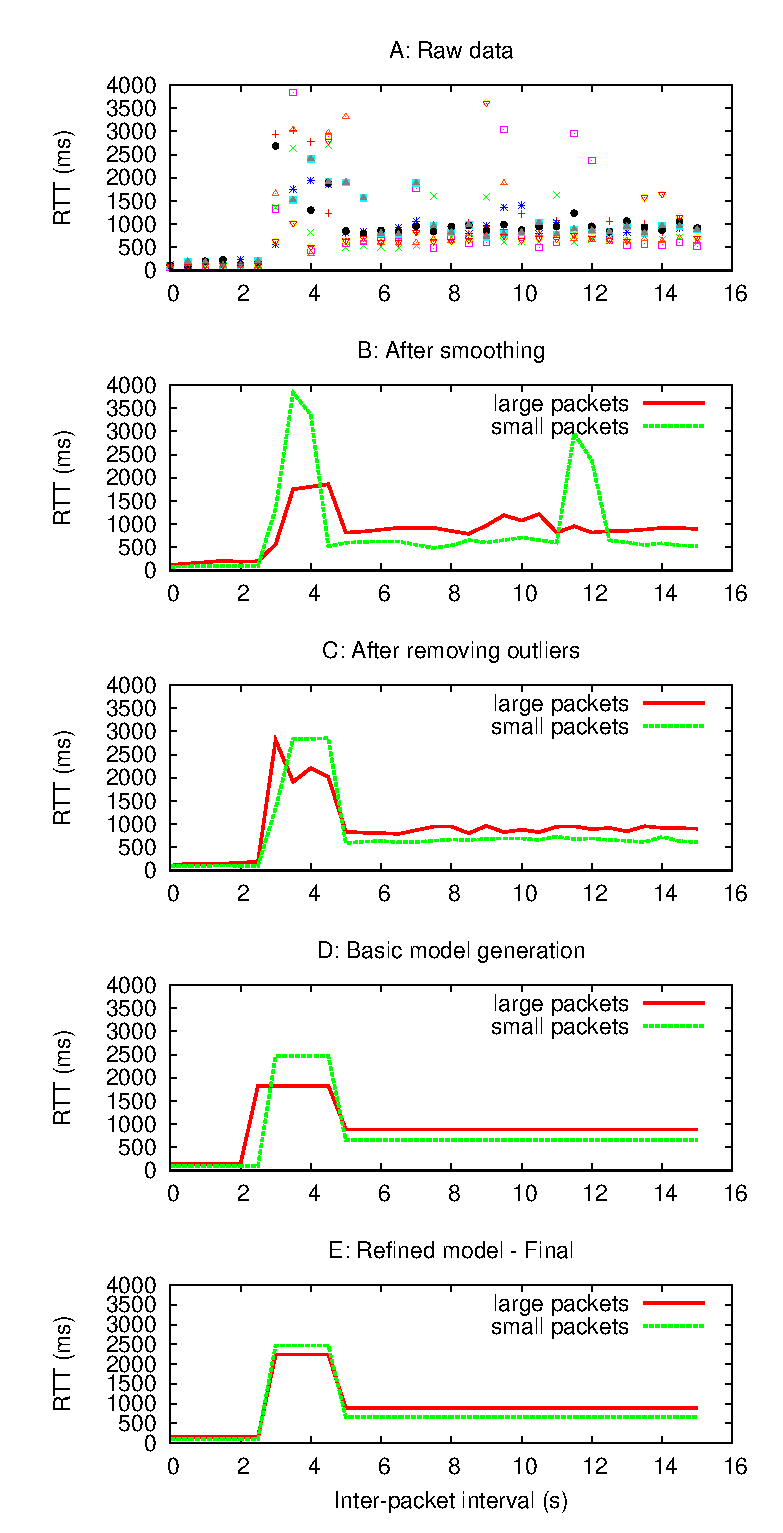
\includegraphics[width=0.5\textwidth]{figs/model_generation.eps}
\end{center}
\ncaption{Steps in extracting RRC model and unexpected behavior trends from raw data.  Note that the raw data follows a non-ideal pattern. Step B: modified running average function that preserves state transitions applied to one test only.  Step C: all tests averaged without outliers removed. Step E: DCH and PCH state extracted; in between them is RRC\_{}TRANSITION rather than FACH --- the anomalous transition period occurs throughout the entire FACH state.}
\label{fig:model_development}
\end{figure}

Aside from storing our results, the server's main role is generating the RRC state models.  Upon uploading a new set of data, a new model is generated for that device ID. To deal with the higher level of noise in our data as well as to be able to analyze all network types and detect unexpected behavior, it was necessary to take an entirely different approach to the server-side analysis from what was done in previous work~\cite{3g_rrc}.

In the ideal case, the data would closely fit the ideal RRC state behavior.  In practice, even in the best case it looks more like Figure~\ref{fig:rtt_raw_data_22}, where there are spikes in latency around RRC transmissions, as well as noise in high-latency RRC states.  There may be far fewer measurements for a device, and the data collected is often noisier. Furthermore, we would like to observe when devices behave in unexpected ways. 

 To create a reasonable RRC model under adverse conditions, we first remove noise from the data, and then divide into timer ranges where RRTs are similar.  Finally, we label the states detected where possible.  We treat 1 KB packets differently from empty packets.  The FACH state is characterized by these packets having very different values and therefore we wish to ensure these differences are preserved.

Filtering noise is not always straightforward, as interesting phenomena such as high round-trip times surrounding state transitions can look like intermittent delays, and vice-versa.  We experimented with several noise filtering approaches on four devices with different manufacturers and carriers to develop our filtering approach before verifying with a larger number of devices.  Taking the average value of all tests was not effective, as these values are often skewed by high amounts of noise.  Taking median values is more effective, but it is also sensitive to periodic noise spikes, especially for small numbers of tests. We also tried taking the minimum value of a set of tests, the intuition being that the network is likely to add delays but not subtract them, but this also resulted in noisy data.

There were two approaches that did work well, however, which are complementary. The first is to remove outliers. If there are three tests, with round-trip times 132, 145 and 370, then most likely the third one is due to intermittent delay.  We disregard all values that are more than half a standard deviation from the mean, or one standard deviation when less than ten tests were performed, then average the remaining values.  This significantly reduces noise in our data in most cases. However, for very noisy data and few tests this still often leaves noise spikes.  If there are three tests, and two coincidentally happen to have latency spikes at the same time, then this spike will not be filtered out.

A modified running average function applied to the data is also effective.  We call this our ``smoothing" function, which is applied to individual tests. For every data point, we first consider the difference between the points on either side of that point.   If this difference is more than a quarter of the data point in question, we leave it as is.  Otherwise, the data point is updated to be the average of the points before and after it. This has two results: first, we filter latency spikes, and second, we do not smooth large jumps in the data which are characteristic of state transitions.

These two approaches complement each other.  Smoothing works well when the probability of a latency spike for each data point is independent, but works poorly where there are consistent RTT delays for several consecutive tests.  Outlier removal works well when a specific test has latency spikes that other tests do not, and especially when a specific test has much longer RTTs than the others. It does not work well for very high levels of random noise.  

After experimenting with various orderings for these two approaches on a number of devices, we found that smoothing each test individually before removing outliers between the tests performs best.  If we remove outliers first, then for noisy data we may inadvertently filter out the correct, low-noise values.  We then smooth the data again at the end to make the data to process cleaner.  The results of these steps can be seen in Figure~\ref{fig:model_development}, parts B and C. B shows the results of smoothing a single test only.

After these pre-processing steps, we create the model. At first, we continue to treat small and large packets separately.  Starting with the smallest interpacket interval, we divide the data into segments with approximately constant round-trip times. The results of this can be seen in Figure~\ref{fig:model_development}, part D.

Then, we compare the two models generated --- that for the large packets, and that for the small packets.  Although the average RTT for the two models differs, the beginning and end of each segment should be the same for both. There are two cases where the boundaries of segments may differ after model generation that need to be corrected.   First, with low amounts of data, it sometimes happens that the beginning and end of a segment for each model is off by half a second.  An example can be seen in Figure~\ref{fig:model_development}, part D. In this case, we find which segment division will result in the smallest average error and apply that to both models.  Second, there are some states where behavior for one packet size or the other does not change.  In particular, in the FACH state it is possible that the RTT for small packets is very close to that in DCH state.  In this case, we split the larger segment.  

Finally, we label the states. We do not use the same assumptions in doing so as in previous work as we find these do not always apply to our data. In particular, we do not assume that in PCH the 1KB packets and empty packets have very similar delays, as we find that this is frequently not the case.  Instead, we determine states based on the relative average RTTs of each segment.  For example, FACH (by definition) has latencies for empty packets close to those in DCH, whereas PCH does not. We also account for the fact that we expect to see states appear in a particular order as we increase inter-packet timings. For example, a carrier implementing the UMTS specification will never demote to FACH after demoting to PCH with no packets being sent.  

This step was first developed and validated on a small number of devices whose behavior was verified using QxDM. It was also validated using an internal deployment on a carrier with known RRC state machine timers.


We look for the following states: high-power (DCH-like), low-power (PCH-like), and FACH-like.  We also look for latency spikes transitioning between these states, like that seen in Figure~\ref{fig:model_development}.  Anything that does not fit one of these patterns we label as ``Anomalous" and flag for manual investigation.  We err on the side of flagging models as anomalous to ensure that all other RRC states are accurate. We describe these results in \S\ref{sec:clientresults}.

%\subsection{LTE Short Timers}
%
%\begin{figure}[t!]
%\begin{center}
%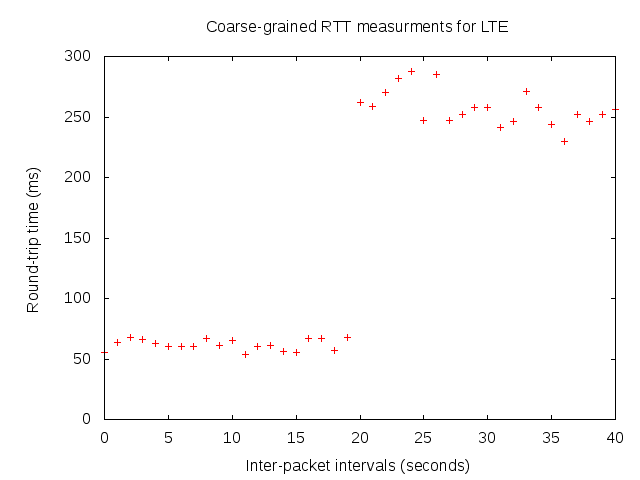
\includegraphics[width=0.45\textwidth]{figs/lte_naive.png}
%\end{center}
%\ncaption{Example data collected for LTE using coarse-grained measurement approach}
%\label{fig:LTE_raw}
%\end{figure}
%
%\begin{figure}[t!]
%\begin{center}
%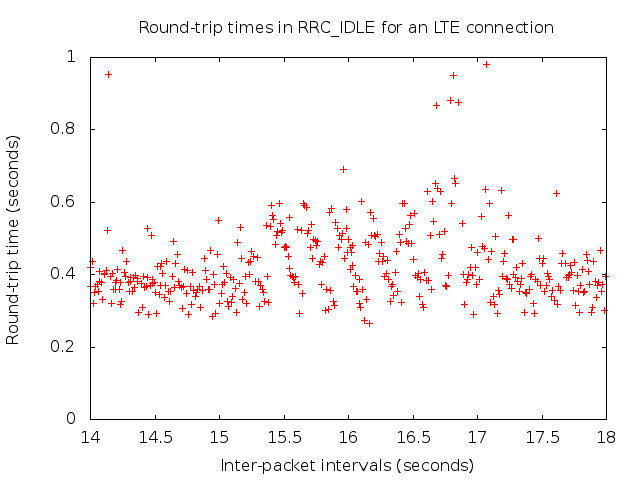
\includegraphics[width=0.45\textwidth]{figs/lte_idle.png}
%\end{center}
%\ncaption{Example data collected for short LTE timers in RRC\_IDLE, focusing on lowest-noise region of test}
%\label{fig:LTE_detailed}
%\end{figure}
%
%
%\begin{figure}[t!]
%\begin{center}
%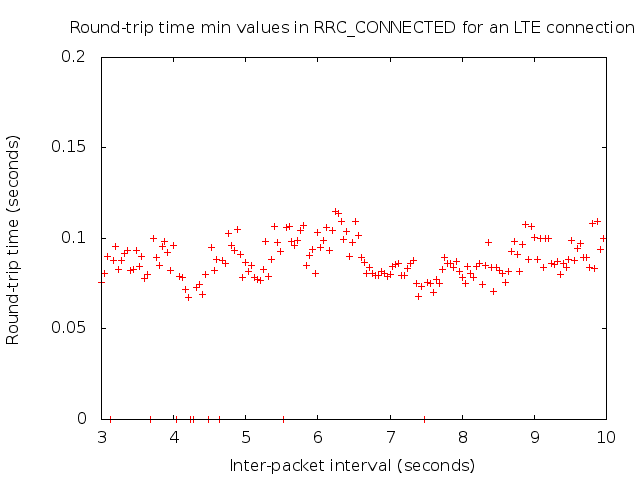
\includegraphics[width=0.45\textwidth]{figs/lte_connected.png}
%\end{center}
%\ncaption{Example data collected for short LTE timers in , focused on }
%\label{fig:LTE_connected}
%\end{figure}
%
%
%This methodology is only suitable for timers at the granularity of half-seconds, evidently.  For 3G this is not a problem, as timers are generally on the order of seconds.  For LTE, the timer for the transition between RRC\_CONNECTED and RRC\_IDLE isisimilarly on the order of seconds. However, as was shown in previous work~\cite{4g_rrc}, some of the timers for the states within RRC\_CONNECTED can be as small as 20 ms, and even the RRC\_IDLE cycle length requires measurements several times a second to detect.  Furthermore, as boundaries for these ``sub-states" are not derived by detecting step functions but rather sawtooth shapes, to accurately detect these timers measurements need to be taken at time intervals several times shorter than the timers that are being inferred.
%
%This introduces a number of challenges, and requires modifications to client-side and server-side code.  We were able to infer timers on the order of 100ms, but probably any on the order of 10ms would not be feasible.
%
%Evidently, it is necessary to send data at much higher frequencies.  Instead of having inter-packet intervals increasing with increments of half-seconds, we have intervals increasing with increments of ten milliseconds.  This does, however, increase the number of tests that need to be done by a factor of fifty, and the length of time needed to complete a single test from tens of minutes to tens of hours.  As a result, we have performed these tests only on devices specifically meant for that purpose.
%
%Additonally, there is the problem that there is a significant amount of jitter on cellular networks, and a great deal of data needs to be collected in order to accurately measure these values. This effect can be seen in Figure~\ref{fig:LTE_raw} --- compare the noisiness of data to that in Figure~\ref{fig:rtt_raw_data_22}.  
%
%A large source of this problem is that delays are introduced due to scheduling and overhead when implemented at the Android Framework level (i.e. in Dalvik).   Both the values collected and the precise length for which the timers run are not accurate to the millisecond. We found that timer values, in particular, are incorrect on average by 3.3 ms, with a standard deviation of 2.8 ms, which could have a substantial impact on timers on the order of 10ms. It is possible to implement our application in C and have it run natively, using the Android NDK.  As a proof-of-concept, we have collected measurements using tcpdump~\cite{tcmpdump} instead, and extract inter-packet timings and RTT values directly. Using this, we were able to eliminate much of the jitter that was preventing us from taking accurate measurements.
%
%Even so, the data we receive can often be quite noisy.  For the idle period in RRC\_IDLE, it suffices to simply perform enough tests that the characteristic sawtooth pattern becomes evident (see Figure~\ref{fig:LTE_detailed}).  In our controlled experiment, one such set of data appeared in our first test performed.  However, for the timers on the order of tens of milliseconds, this is still insufficient.  To recover these, we perform several complete tests, bin inter-packet timings into 10-ms intervals, and take the minimum value of all data points.  This pre-processing step is sufficient to extract these smaller timers, as can be seen in Figure~\ref{fig:LTE_connected}.
%
%Due to the high energy and data cost of these tests, we currently limit them to controlled experiments, and as such in \S~\ref{sec:clientresults} where we perform a large-scale evaluation of global RRC state machines, we focus only on the coarse-grained timers for our LTE measurements.  Crowd-sourcing these timers seems impractical, as the battery cost would probably mean this measurement would not be worthwhile for the average user, but it is certainly possible for an interested expert to infer most LTE timers in this manner. 
%
%\mycomment{Measurements taken with power monitor to verify may suggest these values are not accurate. May change writing to reflect that.}
%
%RRC inference can help us detect new sources of delays, packet loss, and other performance problems, but it does not allow us to understand \emph{why} the unexpected phenomena that we detect occur.  For that, we need to examine lower-level behavior directly.  In the next section, we discuss how we approach this problem and address the issues in understanding RLC-level behavior.
%
%In short, we have significantly improved RRC state inference. We have shown that it is possible to collect network data for RRC inference on arbitrary devices using an application running in the background, without requiring any special expertise, device modifications, or any similar burdens on the users.  We have also found that it is possible to infer very shorty timers associated with LTE states which could not previously be measured.

\section{Cross-Layer Analysis\\Methodology}\label{sec:qxdmresults}

We use QxDM to perform cross-layer analysis for several purposes.  In \S\ref{sec:exp.setup} we describe how we collect ground truth data transmission information in the IP and RLC layers.  We describe the cross-layer mapping algorithm in \S\ref{sec:cross.layer.algo} that allows us to understand the impact of RLC-layer behavior on higher layers, and in \S\ref{sec:rlc.retx.cal} we describe how we calculate the RLC retransmission ratio in QxDM.

%\S\ref{sec:verify.latency} verifies the latency observations using cross layer algorithm.
%\S\ref{sec:ctrl.exp} illustrates the control experiments for further the root cause identification. 

\subsection{QxDM Experiments}\label{sec:exp.setup}

% Describe what the tool does
QxDM is a real-time data collection and diagnostic logging tool for measuring \textit{Radio Frequency} (RF) performance in mobile devices~\cite{qxdm_flyer}. It allows us to gain insight into lower layer RLC transmission information.  
\TReport{It is a Windows based monitoring application. When I perform control experiments and real application measurements, I plug in the device to the desktop or laptop with QxDM software installed. }
The tool was used to collect data on IP packets, RLC data PDUs, and RRC states, as well as RLC control PDUs and RLC configuration information such as polling timers and retransmission limits.  \Paperonly{The experiments performed were done on two devices from two different manufacturers, which we will call M1 and M2.  The M1 device runs Android OS 4.1.1, and the M2 device runs Android OS 4.0.4. This allows us to study potential device-dependent behavior.}

 %We plan to extend this analysis to more device types.
\begin{TReports}
Once the experiments finished, we filtered out the real-time monitoring information related to IP packets, RLC PDUs (protocol data unit, the smallest data transmission unit in RLC layer), and RRC states in Table~\ref{tab:QxDM.logs}, and dumped the results into a log file. The 0x11EB log entry includes IP headers, IP payloads, and its customized header. Since large IP packets will be fragmented into smaller segments, the customer header could indicate the segment index of the whole IP packet. The 0x4132 and 0x4133 unveil the RLC AM (acknowledge mode) configurations, i.e. the polling function timers, the retransmission limit for a single PDU, and etc. The 0x413B, and 0x418B provides RLC PDU header and first byte payload information for both data PDUs and control PDUs (or STATUS PDUs) in both uplink and downlink directions. We wrote a QxDM log parser to aggregate the filtered entries, and apply cross layer analysis to understand the correlation between different layers. We conducted all the experiments on two devices -- Galaxy S3 with Android OS 4.1.1 and HTC One S with Android OS 4.0.4, to observe any device dependent behavior.


QxDM provides precise RRC state information to indicate the current radio channel state. RLC data PDU and status PDU will assist us in cross layer mapping to the transport layer data, i.e. TCP/UDP. Other context information could also be found in the log, i.e. signal strength and physical layer transmission bit rate. The QxDM log is essentially a list of log entries formatted as a uniformed header with timestamp, a detailed log entry description, and a raw hex dump result.  

 Table of QxDM entries
\begin{table}[t!]
\begin{tabularx}{0.5\textwidth}{ | c | X | }
	\hline
  	\textbf{QxDM Log ID} & \textbf{Description} \\
  	\hline\hline
  	0x11EB & IP data packets \\
  	\hline
  	0x4132 & WCDMA RLC downlink acknowledge mode configuration \\
  	\hline
  	0x4133 & WCDMA RLC uplink acknowledge mode configuration \\
  	\hline
  	0x413B & WCDMA RLC uplink acknowledge mode PDU \\
  	\hline
  	0x418B & WCDMA Flexible RLC downlink acknowledge mode PDU \\
  	\hline
  	0x4125 & WCDMA RRC states \\
  	\hline
\end{tabularx}
\ncaption{QxDM log entries used in cross layer analysis}
\label{tab:QxDM.logs}
\end{table}
\end{TReports}

%\subsection{QxDM Experiments}\label{sec:ctrl.exp}

% UDP/ TCP control experiment set up

%\mycomment{To validate our proposed RRC state inference methodology,... Need to say how to validate this}
First, we validate the RRC inference methodology discussed above. We calculate the RRC demotion timers directly from QxDM logs.  According to the 3GPP spec~\cite{spec-3G-RRC}, the sender receives a \textit{radio bearer reconfiguration} (RBR) message from the Node B (\textit{i.e.} the base station) when it demotes from DCH to FACH.  It receives a  \textit{physical channel reconfiguration} (PCR) message upon demoting from FACH to PCH. By measuring the timestamp difference between the last IP packet and the corresponding RBR or PCR message we confirm the inferred RRC demotion timer values.

Second, we wished to investigate the root causes of behavior observed at the UDP layer.  In particular, we wished to uncover the relationship between delays during demotions to and from FACH and RLC-layer transient states. To do so, we ran the RRC inference test for 160 consecutive hours and collected QxDM logs as well as server-side tcpdump~\cite{tcpdump} traces. We labelled our UDP packets with a sequence number, and the echo server sent back the received sequence number.  We refer to this dataset as the \emph{QxDM\_{}UDP\_{}Trace}.  

For a second set of tests, we sent a packet train of TCP packets of size 10 KB with inter-packet timings between 3s and 5s, incremented by 0.5 seconds.  These values were chosen as they fall within the range of inter-packet timings associated with unexpected FACH transition latencies and would allow us to investigate this unexpected behavior. We wished to investigate the RLC retransmission delay's influence on TCP retransmission.  We refer to this dataset as \emph{QxDM\_{}TCP\_{}Trace}.
% TCP contains its own \textit{automatic repeat request} (ARQ) mechanism and w
%The purpose of the control experiments is to verify the unexpected delays over noisy FACH state, and identify the root cause of the problem. First, we repeated our active RRC inference test for 160+ hours and dump both the client QxDM and server side tcpdump traces to perform offline analysis~\cite{tcpdump}. 
%In order to distinguish the identities of each UDP packets, we manually injected a "sequence number" into the first four bytes of the sender's randomized payload, and the echo server sent back the received sequence number as acknowledge number in its payload. We will refer the trace as \emph{QxDM\_{}UDP\_{}Trace} in the later paragraph. Second, we designed a packet train probing using TCP packets so that we could recreate the "pseudo-state" issue~\cite{pkt.train}. Basically, we send a "train" of TCP packet size of 10 KB bytes with interleaving gap period of 3 seconds to 5 seconds incremented by 0.5 seconds with the total of 500 packets. The gap period is the DCH demotion timer period considering the variance in the lossy channel, and adjacent packet will transmit the packet starting from FACH state. Therefore, we will have more transition over the troublesome FACH state to allow us to take a closer look the root cause. Since TCP has its own ARQ (automatic repeat request) mechanism, it would be interesting to investigate the RLC retransmission's delay influence over TCP retransmission. We will refer the trace as \emph{QxDM\_{}TCP\_{}Trace} in the later paragraphs.

% UDP results
%\subsection{Verification Latency using QxDM}\label{sec:verify.latency}

% UDP loss behavior over different states
%QxDM provides the ground truth information about RRC state, so we want to validate the delay behavior based on the inferred RRC model. To verify the packet delay in the transport layer over each RRC state, we need to know the RRC state for transport layer packets and RLC layer PDUs. Since each RRC state log is only a single log entry indicating the change of RRC state, we don't have explicit RRC state information tied to each packet and PDU. Therefore, we determine the RRC states by backtracking the most recent RRC state log, then assign as attributes to the packets and PDUs so that we could acquire RRC state information directly from the packet or PDU itself. 

%Because the the promotion period for PCH and FACH differs from their initial period due to additional signaling overhead, we want to distinguish between a RRC state with and without involving transitions. Since we focus on the initial period of data transmission, the RRC state promotion is more meaningful than state demotion, which is the end of whole data transmission period. So RRC state promotion is our preliminary concern for this project. We break down the normal FACH into an initial FACH state and FACH to DCH promotion state, named as FACH\_{}INIT and FACH\_{}PROMOTE specifically. Similarly, PCH was divided into PCH\_{}INIT and PCH\_{}PROMOTE. Since the FACH promotion timer is on average 0.92 seconds and PCH promotion state is on average 0.21 seconds. We define the FACH\_{}PROMOTE state as the time slot of counting back 0.92 seconds from the point of promoting to DCH. For the same reason, PCH\_{}PROMOTE state describes the time slot of counting back 0.21 seconds from the point of promoting to FACH. 

%From the \emph{QxDM\_{}UDP\_{}Trace}, we calculate the UDP RTT by mapping the client transmitted UDP packets to the served echoed back packets through comparing the manually injected "sequence number". If both packets have the identical "sequence number" in their first four byte payload, then the RTT for the transmitted data is the timestamp difference between the two packets. Figure~\ref{fig:udp.rtt} shows the UDP RTT broken down into different RRC state and state transitions. The average RTT at FACH\_{}INIT state is \textit{2.52 s} for HTC One S and \textit{2.08 s} for Galaxy S3, which around both around \textit{190\%} greater than each one's RTT in DCH. The average RTT for FACH\_{}PROMOTE state is \textit{1.14 s} for HTC One S and \textit{1.05 s} for Galaxy S3, which are around \textit{40\%} greater than those in DCH. The result could validate the abnormal delay behavior especially during the initial part of the FACH state, namely the FACH\_{}INIT state. We could also observe a substantial latency over PCH\_{}PROMOTE state. Because packets cannot stay in PCH during the transmission, the promotion to FACH and DCH will double the signaling overhead, which introduces more latency.

% UDP delay
% RLC Loss ratio per RRC state
%\begin{figure}
%\centering
%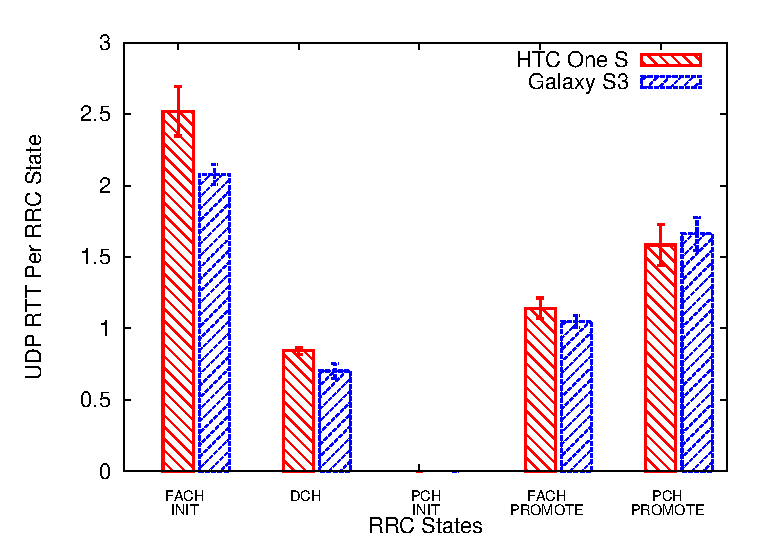
\includegraphics[width=0.5\textwidth]{figs/udp_rtt.eps}
%\ncaption{UDP RTT calculated from the QxDM log result}
%\label{fig:udp.rtt}
%\end{figure}

\subsection{Cross-Layer Mapping Algorithm}\label{sec:cross.layer.algo}

% Describe the mapping algorithm we use for cross-layer analysis
Correlating the transport layer packets with the RLC layer transmitted PDUs would allow us a transparent view of link layer behavior, especially RLC retransmissions.  One major limitation we need to address when using QxDM to analyze data is that packet logging is incomplete. Only the header and first byte of the data payload is logged for each RLC PDU. Furthermore, it is also possible for a small number of RLC PDUs to not be captured, leading to a sequence number gap. We created a mapping algorithm to address these limitations.

% The mapping algorithm here
The cross-layer mapping algorithm maps complete IP packets (known as SDUs, or \textit{Service Data Units}) to the corresponding fragmented RLC payload (or PDU).  PDUs have a fixed size which we denote as $S_{PDU}$.  The basic idea is that we find the first byte of the RLC PDU that matches the first byte of an SDU.  We then skip forward from that byte in the SDU by $S_{PDU}$, and check if that next byte matches the next RLC PDU.  As well, if the sequence number difference $D$ between two consecutive PDUs is greater than 1, then some RLC PDUs are missing from the QxDM trace.  In that case, we skip ahead by $S_{PDU} \times D$ instead.  We know our mapping is complete if every PDU's first byte maps to an SDU, with the SDU bytes being the appropriate distance apart and with the ordering of PDUs and SDUs being conserved.  Otherwise, no mapping was discovered.

%creates a mapping between complete IP packets (also known as SDUs, or \textit{Service Data Units}) and the corresponding fragmented RLC payloads (or the PDUs). The basic idea is that once we find one RLC PDU's first byte matching with the first byte of SDU, then we skip to the next byte at one PDU size away from SDU's first byte to check whether the next RLC PDU's first byte matches that byte. If the sequence number difference (\textbf{D}) between two consecutive RLC PDU is greater than 1, that implies the some RLC PDUs in between were not captured in QxDM. Then we skip the \textbf{D} times of PDU size bytes for SUD in the algorithm. If we map all every PDUs size of byte in SDU to a list of RLC PDU, then we successfully find a mapping; otherwise no mapping was discovered.
 % It is necessary to determine the end of the IP packet associated with each PDU as we iterate over the PDUs. Unfortunately, each PDU can contain either payload data from a single SDU, or from two SDUs.  If an SDU does not fill a PDU then par of the next SDU will be concatenated to fill the rest of the space~\cite{spec-3G-RLC}, to increase transmission efficiency. 
 \TReport{Algorithm~\ref{alg:cross.mapping} describes this mapping mechanism in detail.}
%If the cumulative mapped index equals the size of the SDU (or the length of IP packets), we have successfully found a mapping; otherwise no mapping was discovered.

%is essentially a map between the complete IP packets (known as SDU) and corresponding fragmented RLC payload data bytes (known as PDU). Due to the partial logged information in QxDM, only the first data byte is captured in the log. Thus, we have to skip over the rest of the PDU, and try to match for the first data byte in the next PDU. The problem at this point is to determine the end of IP packets while we iterate through the consecutive RLC PDUs. Since each PDU could either contain the payload data dedicated to a single SDU or belongs to two SDUs. If the reminder size of the SDU cannot fulfill the largest size of PDU, then RLC protocol will concatenate the part of the next SDU to fill the rest of space~\cite{spec-3G-RLC}. Ultimately, if the accumulative mapped index equals the size of SDU, we claim to find a mapping successfully; otherwise no mapping discovered. Algorithm ~\ref{alg:cross.mapping} states the detailed information of the mapping mechanism.

% the corner case of the mapping algorithm
% --- this is respesented by the ``factor" variable in the mapping algorithm.  %Sanae: this factor isn't actually mentioned any more.
However, this mapping mechanism cannot recover all packets in every case. In particular, this is true when missing PDUs are at the beginning or end of the mapped RLC list, but those cases occur rarely in the QxDM traces. We evaluate the accuracy of this improved mapping algorithm by observing the percentage of mapped IP packets in both the \emph{QxDM\_{}TCP\_{}Trace} and the \emph{QxDM\_{}TCP\_{}Trace}. We were able to correctly map 99.8\% of packets. 

%\mycomment{besides using mapping coverage as a metric for evaluation, what are other ways we can validate the correctness of the mapping? Answer: another way to validate the mapping is to map group of RLC PDU back to the TCP/UDP packets, but due to missed log information, we are not 100\% confidence in that direction.}

%There is a corner case in the mapping algorithm such that the QxDM cannot capture the some of the SDUs. Similar to TCP protocol, the sequence number in RLC PDUs could uniquely distinguish between every PDUs. If there are some missed PDUs, then we cannot map the first byte data for every PDU size. In that case, we could even skip over the missed PDUs and add up multiple of PDU size to hunt for a match, which is represented as "factor" variable in the mapping algorithm. However, the aggressive leap mapping mechanism cannot fully recover the corner case, especially when the missed PDUs were either the beginning or the end part of the mapped RLC list. We evaluate the improved mapping algorithm by checking the percentage of mapped IP packets in all the traces of control experiments, and the average mapping ratio is \textit{99.8\%}.

% algorithm detail
\begin{TReports} 

\begin{algorithm}[t!]
\begin{algorithmic}[width=0.5\textwidth]
\STATE {\textit{\textbf{Function} Cross-Layer-Mapping(SDU, PDU\_{}LIST):}}
\STATE {// point to the current mapped PDU in \textit{PDU\_{}LIST}}
\STATE {Initialize \textit{PDU\_{}INDEX} as $0$}
\STATE {// point to the current mapped byte in SDU)}
\STATE {Initialize \textit{SDU\_{}MAPPED\_{}INDEX} as $0$}
\STATE {Initialize \textit{MAPPED\_{}PDU\_{}LIST} as empty list}
\WHILE {PDU\_{}INDEX is less than length of PDU\_{}list}
\WHILE {\textit{SDU\_{}MAPPED\_{}INDEX} $<$ SDU size}
\IF {\textit{SDU[SDU\_{}MAPPED\_{}INDEX]} equals to \textit{CUR\_{}PDU}}
	\STATE {// Success to map current byte}
	\STATE {Append \textit{CUR\_{}PDU} to \textit{MAPPED\_{}PDU\_{}LIST}}
	\STATE {\textit{CUR\_{}PDU} = \textit{PDU\_{}LIST[PDU\_{}INDEX]}}
	\STATE {$factor$ is seq\_{}num between \textit{CUR\_{}PDU} and \textit{LAST\_{}PDU}}
	\STATE {Set \textit{LAST\_{}PDU} as \textit{CUR\_{}PDU}}
	\IF {\textit{cur\_{}PDU} has LI field in header}
		\STATE {Increase \textit{SDU\_{}MAPPED\_{}INDEX} by the value of LI field}
	\ELSE
    		\STATE {Increase \textit{SDU\_{}MAPPED\_{}INDEX} by the size of \textit{CUR\_{}PDU} multiples $factor$}
    	\ENDIF
    	\IF {\textit{CUR\_{}PDU}'s HE field indicate last PDU}
    		\STATE {Break}
    \ENDIF
\ELSE
	\STATE {// fail to map the current byte}
	\STATE {Reset \textit{MAPPED\_{}PDU\_{}LIST} as empty list}
	\STATE {Reset \textit{SDU\_{}MAPPED\_{}INDEX} as $0$}
	\STATE {Break}
\ENDIF
\STATE {Increase \textit{PDU\_{}INDEX} by $1$}
\ENDWHILE
\IF {\textit{SDU\_{}MAPPED\_{}INDEX} equals to SDU size}
	\STATE {// Success to find a mapping!}
	\RETURN {\textit{MAPPED\_{}PDU\_{}LIST}}
\ENDIF
\ENDWHILE
\RETURN {\textit{NOT FOUND}}
\end{algorithmic}
\caption{Map the SDU to the corresponding PDU list}
\label{alg:cross.mapping}
\end{algorithm}

\end{TReports} 

\subsection{RLC Retransmission Calculation}\label{sec:rlc.retx.cal}

The RLC layer includes a retransmission mechanism to improve the reliability of transmissions over the lossy data transmission channel.  However, this may not eliminate unnecessary retransmissions,  as it acts independent of upper layers. This is especially problematic for TCP retransmission timeouts. We describe in this section how we determine when RLC retransmission has occurred from the QxDM logs.

%The RLC layer retransmission is a protection mechanism that maximize the reliability over a loss data transmission channel. However, it also causes the delays due to duplicate transmissions without noticing the upper layers. To assist further identifying the root cause of the latency, we first introduce how we calculate the RLC retransmission from the QxDM logs.

% how to calculate the RLC retransmission
Each RLC sequence number uniquely identifies each RLC PDU, so we can determine RLC retransmissions based on duplicate sequence numbers.  One complication is that sequence numbers wrap around every 4096 PDUs.  To avoid over-counting duplicate sequence numbers from a different cycle, a window size of 512 PDUs is set to count how often sequence numbers reappear. The number of RLC retransmissions is the cumulative count of the repeated sequence number for a given list of RLC PDUs~\cite{spec-3G-RLC}.

% RLC retransmission Ratio calculation
The RLC retransmission ratio measures the relative frequency of RLC retransmissions over a range of time as defined in Table ~\ref{tab:terminology}. First, we describe how to determine the retransmission ratio for a RRC state. The RRC state for each RLC PDU is determined by backtracking to the most recent RRC state QxDM log entry. RLC-layer retransmitted PDU counts are broken down based on the RRC states where they were transmitted. By dividing the total number of retransmitted PDUs by the total number of PDUs in each RRC state, the retransmission ratio can be calculated. We also calculate the RLC layer retransmission ratio for specific inter-packet times (as described in \S\ref{sec:methodology}) by  counting retransmissions over a certain inter-packet time transmission period.

%The sequence number of the RLC PDU will uniquely identify each RLC packet. Therefore, we determine the RLC retransmission based on the duplicate of sequence numbers. Since the size of RLC PDU is only 42 bytes and is very limited, if the RLC keeps an effective throughput, it has to reduce the number of bits in the header to hold the sequence number. Therefore, the sequence number only consumes 12 bits (range of 0-4095) in the current RLC protocol~\cite{spec-3G-RLC}. As a result, sequence number is circularly reused every 4096 PDUs, and it is always increasing. To avoid over-count the duplicate sequence number in different cycle, we hard set a smaller window size of 512 to count the reappearing sequence number within that range. We determine the RRC state for each RLC PDU by backtracking to most recent RRC state log entry, and fetch the RRC state based on that log content. We break down RLC retransmitted PDUs based on their RRC states when they were transmitted, and we calculate the retransmission ratio through dividing total number of retransmitted PDUs per RRC state by the total number of PDUs in that RRC state.

\section{Evaluation Results}\label{sec:clientresults}

\begin{table*}[th!]\small
\begin{tabularx}{\textwidth}{|c|c|c|X|}
\hline
\textbf{\S} & \textbf{Figures \& Tables} & \textbf{Data Source} & \textbf{Description} \\
\hline
\ref{sec:controlledexperiments} & Table~\ref{tab:tmobile_rrc_state} & Controlled experiments using \TReport{T-Mobile devices}\Paperonly{carrier C1} & RRC state timers inferred \\
\hline
\ref{sec:controlledexperiments} & Figure~\ref{fig:all_carrier_rrc_delays} & Controlled experiments using \TReport{T-Mobile devices}\Paperonly{carrier C1} & Unexpected high-latency transitions detected; behavior device-dependent \\
\hline
\ref{sec:controlledexperiments} & Table~\ref{tab:extra_tests} & Controlled experiments using \TReport{T-Mobile devices}\Paperonly{carrier C1}  & Impact on higher-layer protocols measured. DNS, TCP handshakes affected by RRC state; HTTP independent\\
\hline 
\ref{sec:qxdm.analysis} & Table~\ref{tab:tmobile_rrc_state} & \emph{QxDM\_{}TCP\_{}Trace} \& \emph{QxDM\_{}UDP\_{}Trace} & RRC state timer validation in QXDM \\
\hline
\ref{sec:qxdm.analysis} & Figure~\ref{fig:udp.rlc.prove}, Figure~\ref{fig:RLC.Loss.Per.RRC.UDPTrace}, Figure~\ref{fig:RLC.Dup.Ack} & \emph{QxDM\_{}TCP\_{}Trace} \& \emph{QxDM\_{}UDP\_{}Trace} & Root cause analysis of unexpected latencies using cross-layer mapping mechanism \\
\hline 
\ref{sec:qxdm.analysis} & Figure~\ref{fig:udp.loss}, Figure~\ref{tab:udp.loss.root.cause} & \emph{QxDM\_{}UDP\_{}Trace} & Analyze root cause of UDP packet loss behavior \\
\hline 
\ref{sec:largescalestudy} & Figure~\ref{fig:timer_cdf} & Public deployment &  Inferred RRC implementations globally; varies by carrier\\
\hline
\ref{sec:largescalestudy} &  Figures~\ref{fig:all_carrier_rrc_delays} and Figure~\ref{fig:loss_compare} & Public deployment & Confirm delays and losses during state transitions a common problem \\
\hline
\ref{sec:largescalestudy} & Figure~\ref{fig:device_compare} & Public deployment & Device-dependence of RRC performance\\
\hline
\end{tabularx}
\ncaption{Summary of key results}
\label{tab:result.summary}
\end{table*}

First, we describe our findings from our client-based RRC inference approach applied to devices applied to devices in controlled experiments, and next describe how we used QxDM-based cross-layer analysis to verify our findings and investigate root causes of our observations, in particular the impact of transient states.  Next, in \S\ref{sec:largescalestudy} we describe the results of the public deployment of our inference tool to examine the representativeness of our findings for RRC states worldwide. Our results are summarized in Table~\ref{tab:result.summary}.  For privacy reasons, we anonymize all data that might identify users when collecting data\Paperonly{, and anonymize the names of all devices and carriers in describing our results}.

%We took two main types of RRC inference-related measurements.  First, we took measurements in a controlled setting, using a set of custom RRC inference tools. There were two main components of these tests that we describe below:  a controlled deployment within T-Mobile of our client-based inference tool on experimental devices, and a set of experiments on local devices requiring QxDM analysis.  Our preliminary tests to develop the RRC inference algorithm were described in \S\ref{sec:stateinferencemethodology} and we do not repeat them here.

%Second, we also deployed a pared-down version of our coarse-grained timer inference tool in order to understand global trends in RRC state machine behavior. The most important difference between that tool and our internal tool is that our internal tool always perform a complete set of tests, whereas the widely-distributed version may take an incomplete set of measurements if there is a loss of cellular connectivity (for example, if the device switches to WiFi.) These tests allow us to understand trends in RRC state implementations and performance around the world, and how they differ by carrier, device model and network technology.We describe the results of these tests in \S\ref{sec:largescalestudy}.


\subsection{Controlled Experiments}\label{sec:controlledexperiments}

We collected three types of data from our controlled experiments: results from a small number of test devices on various carriers, to develop and validate our analysis methodology; \Paperonly{results from a deployment within a large U.S. carrier we call \emph{C1}}\TReport{results from a deployment within T-Mobile}, to measure RRC states and performance characteristics; and results from QxDM traces to validate the \Paperonly{C1}\TReport{T-mobile} results and investigate root causes of the phenomena we detected.  %The results of our first set of tests were confirmed with power monitor measurements as well as through discussions with Carrier C1 to verify our findings.  
We primarily discuss the second two sets of results in this section.

The inference measurements from the \Paperonly{C1}\TReport{T-mobile} deployment are shown in Table~\ref{tab:tmobile_rrc_state}. These timers have changed since being measured in previous work~\cite{3g_rrc}, underscoring the usefulness of a tool that can be used to crowdsource the taking of continuous measurements.   What is of particular interest is the increase in latency when transitioning from DCH to FACH for UMTS. This latency generally lasts from 1 to 2.5s.  A similar pattern was occasionally seen when promoting to DCH, but generally lasts no more than half a second.  Likewise, this delay sometimes occurred in LTE when demoting to RRC\_{}IDLE, although it was only observed in our public deployment. An example of this phenomenon can be seen in Figure~\ref{fig:rtt_raw_data_22}.  This delay is of particular concern because the associated RTTs are often significantly longer even than those in PCH. In some cases, the user derives no benefit from the low-power FACH state at all, as this phenomenon lasts long enough that the expected FACH behavior is never observed.

%Using our internal deployment, we found that the timers and state machines were consistent for devices in several locations across the U.S.  We focused primarily on measuring demotion timers and performance in each RRC state. For LTE, we found a timer of 10s to transition from the high-power to low-power state.  We did not find any transition delays in LTE for our controlled study, likely because of the limited number of devices, as devices in our public study exhibited this behavior. For standard UMTS, we found a 2.5s timer to demote to FACH and another 2.5s timer to demote to PCH, and also detected a period of high latency when demoting from DCH to FACH, lasting from 1 to 2.5s. In other words, in some cases, this phenomena prevented any performance gains from using FACH. There were a small number of devices on an EDGE network, from which we detected two demotion timers demotion timer of 2.5s between the low-power and high-power state, with no intermediate state detected.  A single device on HSDPA had a timer of 2.5s to demote to the low-power state, also with no intermediate state.  % ALL VALUES FINAL

%There is a second RRC state machine deployed in some locations for 3G that we did not detect. 


%Figure~\ref{fig:network_tech_compare} summarizes the difference between UDP RTTs for different RRC states.  We classify DCH and RRC\_{}CONNECTED, for 3G and 4G technologies, as high power; IDLE and RRC\_{}IDLE as low-power, and FACH as medium-power.  The RTT spike when transitioning from DCH to FACH is indicated as ``transition", and for this carrier occured only for UMTS. No error bars are shown for HSDPA since we only have one set of measurements for this technology.  

%In general, performance improves slightly for newer technologies, especially when going from DCH to FACH. Consistent with previous work~\cite{4g_rrc}, improvements in latency between LTE and 3G technologies are not dramatic. It was found in previous work that is mostly bandwidth where LTE benefits, and the largest improvements are in the low-power state for large packets, albeit with a very high variance in our measurements.  It can be seen clearly here that the worst performance (aside from EDGE) is in the transition period between DCH and FACH, and furthermore that the average latency for small packets in FACH is not substantially better than in PCH.

%TODO: higher-level protocols
%TODO: measure latency again


%\begin{figure}[t!]
%\begin{center}
%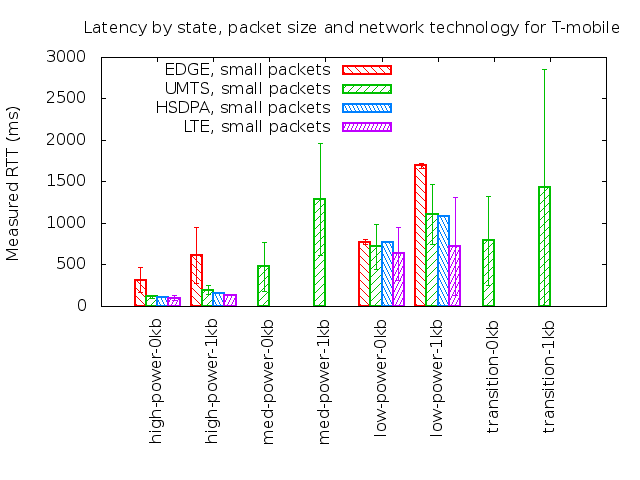
\includegraphics[width=0.45\textwidth]{figs/network_tech_compare.png}
%\end{center}
%\ncaption{Performance of Various Network Technologies for a Single Carrier (T-Mobile)}
%\label{fig:network_tech_compare}
%\end{figure}

We examined the impact of RRC state on several higher-level protocols as well.  We investigated the time to complete a DNS lookup, a TCP handshake, and the loading of a small webpage over HTTP to illustrate the impact of promotion overhead.  For the DNS test, we generated a random, invalid URL, as we found that on some devices the DNS cache could not be flushed.  For TCP, we measured the time to perform a TCP handshake with \url{www.google.com}, and we measured the time to access \url{www.google.com} through HTTP. The results are summarized in Table~\ref{tab:extra_tests}.

In general, there was a very high variance for the data collected in each of the states. TCP handshakes and DNS lookups, like raw UDP packets, appear to be affected by the RRC state of the initial packet sent, in large part because these tests involve few packets.  For HTTP, however, the impact of the starting RRC state was not statistically significant.  This is also unsurprising, as the RRC state only affects the first packet sent.  FACH\_{}TRANSITION appears to have a performance impact, however. RRC state would primarily impact frequent, low-bandwidth transmissions, such as applications that perform periodic polling, as observed in previous work~\cite{aro}. 

\begin{table}[t!]\small
\begin{tabularx}{0.5\textwidth}{|X|X|X|X|X|}
\hline
\textbf{Network Type} & \textbf{DCH/ RRC CONNECTED (s)} & \textbf{FACH (s)} & \textbf{Transition delay?} & \textbf{\# devices observed}\\
\hline \hline
UMTS & 3 & 2 & Yes* & 12 \\
\hline
HSDPA & 3 & None & No & 1 \\
\hline
LTE & 10 & None & No & 3 \\
\hline
EDGE & 2 & None & No & 3 \\
\hline \hline
\multicolumn{5}{|c|}{\textbf{QxDM Ground Truth}} \\
\hline\hline
UMTS & 3.2 & 2.3 & Yes & 2 \\
\hline
\end{tabularx}
* For a subset of devices
\ncaption{Inferred timers for controlled experiments on a major US carrier; ground truth for UMTS from QxDM} 
\label{tab:tmobile_rrc_state}
\end{table}

\begin{table}[t!]\small
\begin{tabularx}{0.5\textwidth}{|X|X|X|X|X|}
\hline
\textbf{Protocol} & \textbf{DCH (ms)} & \textbf{FACH TRANSITION (ms)} & \textbf{FACH (ms)} & \textbf{PCH (ms)} \\
\hline \hline
DNS lookup (UDP)& 449 $\pm$ 881  & 1656 $\pm$ 1157 & 776 $\pm$ 948 & 1209 $\pm$ 1350 \\
\hline
TCP handshake & 229 $\pm$ 191 & 1524 $\pm$ 1371 & 1114 $\pm$ 1096 & 936 $\pm$ 674 \\
\hline
HTTP & 3120 $\pm$ 6465 & 3530 $\pm$ 4905 & 2926 $\pm$ 1609  & 3338 $\pm$ 6031 \\
\hline
\end{tabularx}
\ncaption{Comparison of 3G performance across different RRC states for higher-level protocols. FACH TRANSITION refers to a period of high latency when packets are sent during promotions to FACH due to RLC-layer transient state behavior. Note RRC state dependence of DNS and TCP in particular.}
\label{tab:extra_tests}
\end{table}

%\begin{figure}
%\begin{center}
%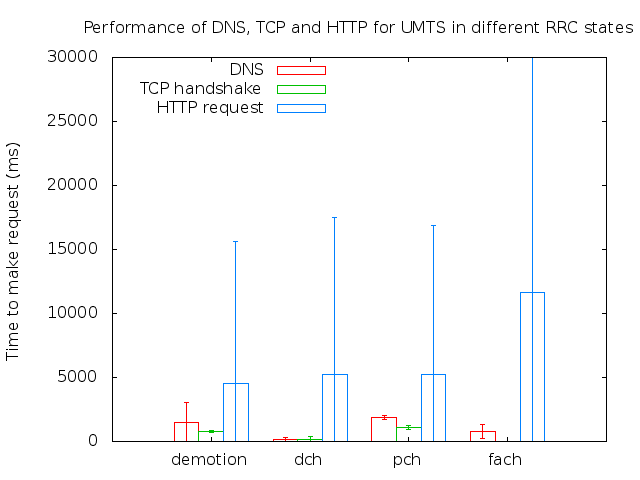
\includegraphics[width=0.45\textwidth]{figs/extra_tests.png}
%\end{center}
%\ncaption{Impact of RRC state on non-UDP protocols}
%\label{fig:extra_tests}
%\end{figure}

\subsubsection{Cross-Layer Root-Cause Analysis with QxDM}\label{sec:qxdm.analysis}
% TODO: include the infered timer part here
We first validate the inferred RRC timers using the method described in \S\ref{sec:exp.setup}. The time difference between the last IP packet and the associated RBR message is around 3.2 seconds. Similarly, the PCH demotion timer is approximately 2.3 seconds, based on the time difference between the last IP packet in FACH and the associated PCR message. The first timer result matches the one in Table~\ref{tab:tmobile_rrc_state} exactly, rounding to the nearest half-second (as that is the granularity at which the measurements were taken). The second timer matches closely as well.

Next, we examine the root cause of the unexpected latencies when transitioning between RRC states. We make use of data from \emph{QxDM\_{}UDP\_{}Trace} and \emph{QxDM\_{}TCP\_{}Trace}.
%, and in \S\ref{sec:eval} we propose an approach to avoid these unexpected latencies.  We also identify the prevalence and root causes of UDP packet losses. In this section, 
Making use of the terminology defined in \S\ref{sec:background}, we examine each of the \emph{transient states} at the RLC layer to understand the root causes of this behavior.  Based on our measurements of the FACH and PCH promotion times, we determine that FACH\_{}PROMOTE covers the time period of 0.92 seconds before promotion to DCH occurs in \emph{QxDM\_{}UDP\_{}Trace} and \emph{QxDM\_{}TCP\_{}Trace}. Similarly, PCH\_{}PROMOTE covers the time period of 0.21 seconds before FACH promotion occurs as defined in Table~\ref{tab:terminology}.

%We identify the root cause of unexpected latencies by making use of results from a set of QxDM measurements that we will refer to as \emph{QxDM\_{}Trace}.  We propose in \S\ref{sec:eval} an approach to avoid these unexpected latencies.  Next, we use \emph{QxDM\_{}Trace} to identify the prevalence and root causes of UDP packet losses.  

%\S~\ref{sec:root.cause.analysis} identifies the root cause of latency by results from both emph{QxDM\_{}Trace}, and propose RLC Fast retransmission mechanism to reduce the RLC delay. \S~\ref{sec:udp.loss.analysis} is a case study of utilizing the cross-layer mapping and retransmission calculation technique to identify the root cause of the UDP packet loss.
%\subsection{Cross-Layer Analysis with QxDM}\label{sec:qxdm.analysis}
%\S~ref{sec:rrc.term} defines and highlights subset of FACH state so that we could have fine grained understanding the abnormal latency issue. \S~\ref{sec:root.cause.analysis} identifies the root cause of latency by results from both emph{QxDM\_{}Trace}, and propose RLC Fast retransmission mechanism to reduce the RLC delay. \S~\ref{sec:udp.loss.analysis} is a case study of utilizing the cross-layer mapping and retransmission calculation technique to identify the root cause of the UDP packet loss.

%However, as at the RLC layer we can observe various phenomena that are not detectable at higher layers, we will start by defining some terminology. Because the the promotion period for PCH and FACH differs from their initial period due to additional signaling overhead, we want to distinguish between a RRC state with and without involving transitions. Since we focus on the initial period of data transmission, the RRC state promotion is more meaningful than state demotion, which is the end of whole data transmission period. So RRC state promotion is our preliminary concern for this project. We break down the normal FACH into an initial FACH state and FACH to DCH promotion state, named as FACH\_{}INIT and FACH\_{}PROMOTE specifically. Similarly, PCH was divided into PCH\_{}INIT and PCH\_{}PROMOTE.

%Since the FACH promotion timer is on average 0.92 seconds and PCH promotion state is on average 0.21 seconds, we consider the time
%define the FACH\_{}PROMOTE state as the time slot of counting back 0.92 seconds from the point of promoting to DCH. For the same reason, PCH\_{}PROMOTE state describes the time slot of counting back 0.21 seconds from the point of promoting to FACH.

%\subsubsection{Root Cause of Latency}\label{sec:root.cause.analysis}
% explain why we want to calculate RLC layer retransmission and how to calculate

To demonstrate the strong correlation between data link layer retransmissions and higher layer latencies, we calculate the RLC layer retransmission ratio for each inter-packet time interval using the methodology described in \S\ref{sec:rlc.retx.cal}. We insert the inter-packet time for the test performed in the packet payload for data in the \emph{QxDM\_{}UDP\_{}Trace}, so we can directly correlate the RLC PDUs with the associated inter-packet timing after we apply the cross-layer mapping algorithm from \S\ref{sec:cross.layer.algo}. In Figure~\ref{fig:rlc.retx.gap} the high retransmission ration in FACH can be seen, which matches the latency behavior in Figure~\ref{fig:udp.rtt.gap}. The similar patterns imply that the root cause of the FACH latency issue resides in the data link layer.

\begin{figure}[t!]
\centering
%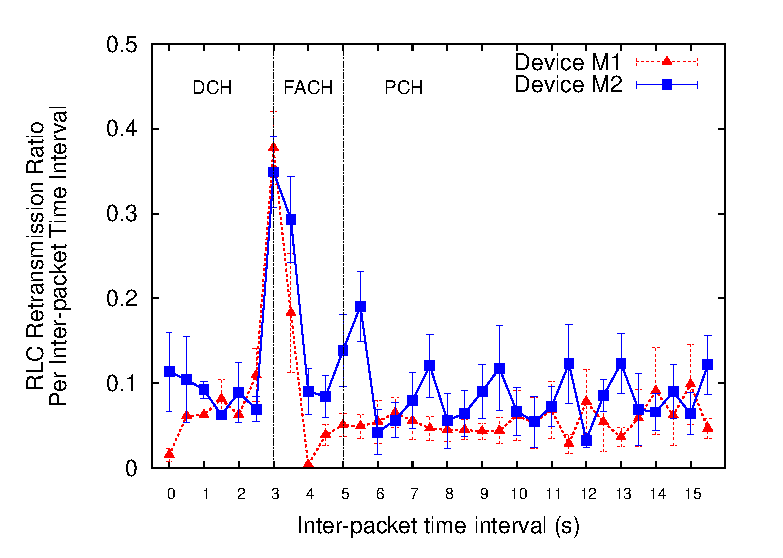
\includegraphics[width=0.5\textwidth]{figs/rlc_retx_gap.eps}
%\begin{subfigure}
%\centering
%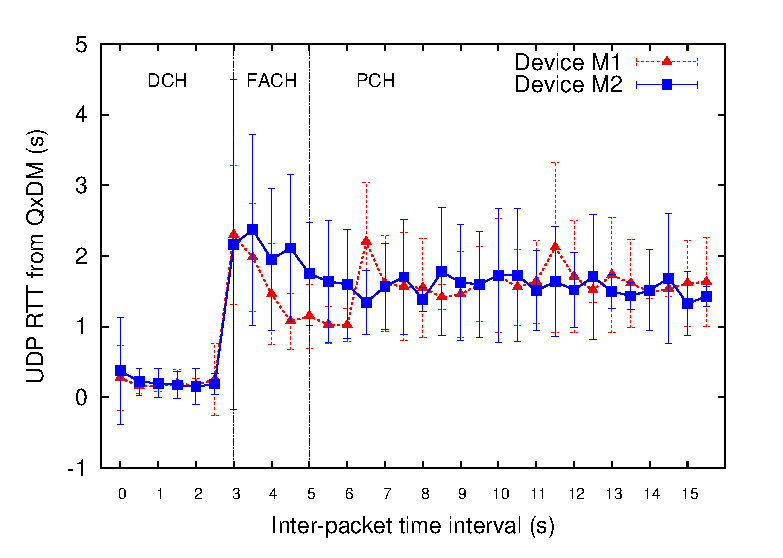
\includegraphics[width=0.5\textwidth]{figs/udp_rtt_gap.eps}
%\label{fig:udp.rtt.gap}
%\end{subfigure}%
%\begin{subfigure}{0.5\textwidth}
%\centering
%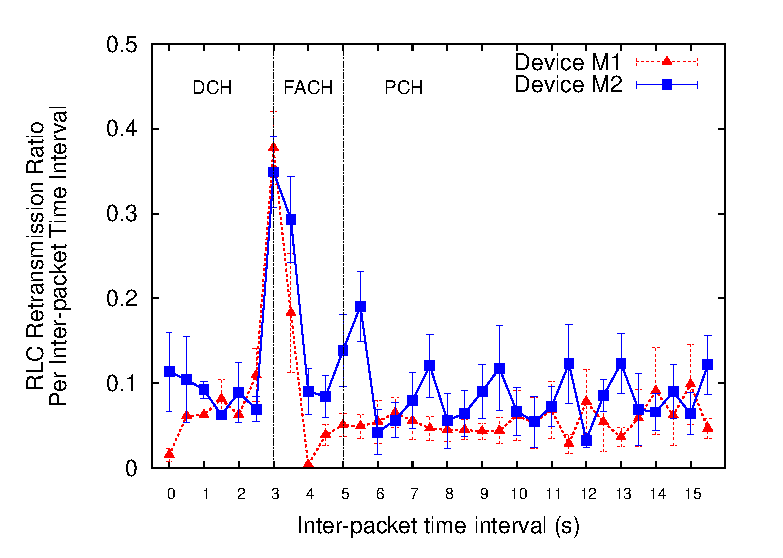
\includegraphics[width=0.5\textwidth]{figs/rlc_retx_gap.eps}
%\label{fig:rlc.retx.gap}
%\end{subfigure}
\subfigure[UDP RTT Result]{\label{fig:udp.rtt.gap}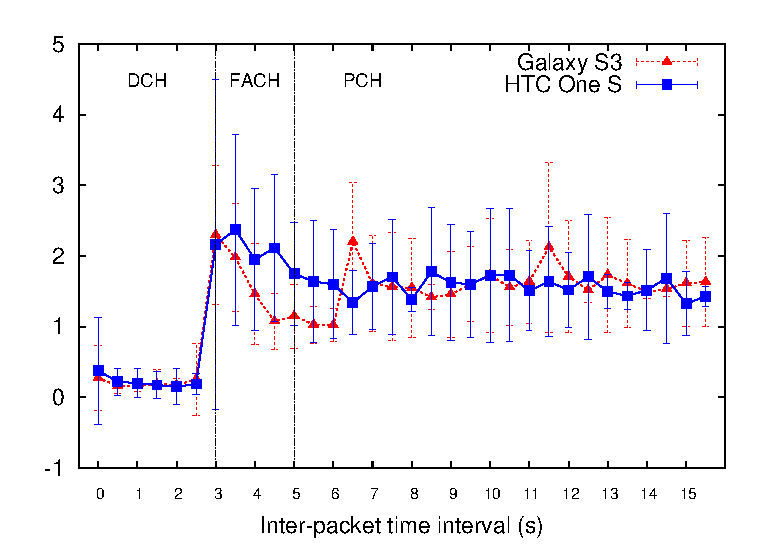
\includegraphics[width=0.5\textwidth]{figs_nonanony/udp_rtt_gap.eps}}\\%
\vspace{-3.0ex}
\subfigure[RLC Retransmission Result]{\label{fig:rlc.retx.gap}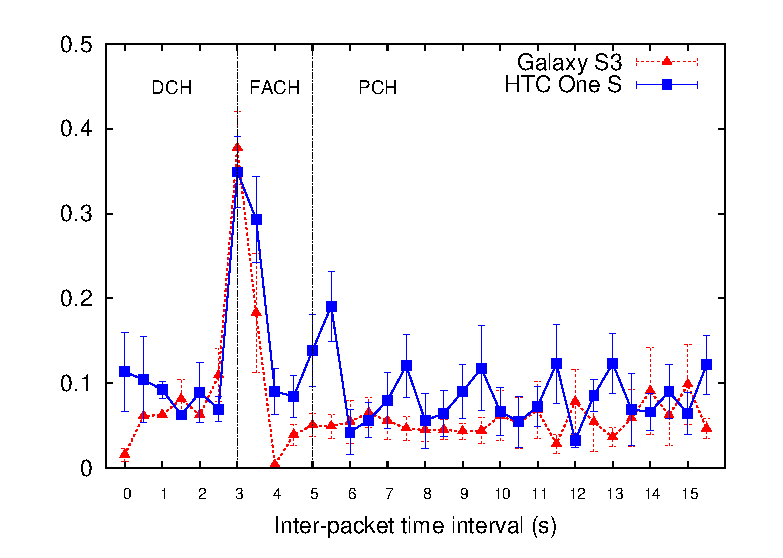
\includegraphics[width=0.5\textwidth]{figs_nonanony/rlc_retx_gap.eps}}%
\ncaption{RLC layer retransmission ratio has a strong correlation with the delay over FACH state. Measurements on 1 KB packets.}
\label{fig:udp.rlc.prove}	
\end{figure}

There are two possible RLC retransmission behaviors that lead to delays at the transport layer. First, retransmission may be necessary due to noisy channel conditions during FACH. Based on the \emph{QxDM\_{}UDP\_{}Trace} and the \emph{QxDM\_{}TCP\_{}Trace}, we can see that RLC retransmission ratios are particularly high during FACH.  A possible solution to this problem is for the application to batch data transmissions to reduce the frequency of RRC state promotions, a solution that has been shown to be beneficial in eliminating other transmission-related delays~\cite{3g_rrc}.  Second, retransmissions can become unnecessarily delayed due to a slow response to the PDU loss signal (i.e., duplicated ACKs). In particular, this can effect TCP transmissions, as the relationship between TCP retransmissions and RLC retransmissions leads to delays.  We propose a solution to address this latter problem in \S\ref{sec:eval}.

%a strong correlation between RLC retransmission ratio and FACH state as an evidence. One possible solution is that application could batch the data transmission to reduce the RRC state promotion frequency~\cite{3g_rrc}. The second one is the retransmission get unnecessary delayed caused by the lagging response to the PDU loss signal. We also observe it from \emph{QxDM\_{}Trace} when we studied the relationship between TCP retransmission and RLC retransmission. We will also provide a improved RLC mechanism to avoid the unnecessary delay later.

% UDP trace analysis

Using the RLC retransmission calculation methodology described in \S\ref{sec:rlc.retx.cal}, we calculate the RLC transmission ratio for each transient state. We show these results in Figure~\ref{fig:RLC.Loss.Per.RRC.UDPTrace}. The retransmission ratios are particularly high in FACH\_{}INIT and FACH\_{}PROMOTE. For the \Paperonly{M2}\TReport{HTC} device, the ratio is especially high during FACH\_{}INIT. These observations are consistent with the abnormal delays we observed when transitioning from DCH to FACH at the UDP layer. The higher loss rates for the device made by \Paperonly{M2}\TReport{HTC} are consistent with the differences between devices found in the public study in \S\ref{sec:largescalestudy}. A possible explanation is the difference in hardware used. \Paperonly{The M1 and M2 devices use two different generations of chipsets, and the newer one  supports a larger range of network types}\TReport{The HTC device uses Snapdragon S3 MSM8260, while the Galaxy S3 contains the next-generation Snapdragon S4 MSM8960 and supports a larger range of network types}~\cite{snapdragon}. This chipset dependency might also explain why this phenomenon was not observed in earlier work, on older devices, which likely used yet another chipset. In our public study we found that there are a number of chipsets from various companies that exhibit this behavior. However, a detailed examination of hardware differences is out of the scope of the paper.

%HTC device uses Snapdragon S3 MSM8260, while the Galaxy S3 contains the next-generation Snapdragon S4 MSM8960 and supports a larger range of network types~\cite{snapdragon}. This 

%Analyzing the \emph{QxDM\_{}Trace} based on the RLC retransmission calculation methodology, we calculate the RLC retransmission ratio per RRC state in Figure~\ref{fig:RLC.Loss.Per.RRC.UDPTrace}. As we can see, the RLC retransmission among FACH and FACH\_{}PROMOTE in total are \textit{46.63\%} for HTC One S device with standard deviation of \textit{4.28\%}, and \textit{14.23\%} for Galaxy S3 devices with standard deviation of \textit{0.66\%}. It strongly suggested the significant delay over the FACH\_{}INIT and FACH\_{}PROMOTE states, which indicates the higher chance of RLC retransmission in a resource shared and noisy channel during FACH state. The observation is consistent with the abnormal delays during initial FACH state as we could also observe radio bearer configuration signaling and other system signaling exchange between the handset and the base station. We also observe that the HTC device has a higher loss rate than that of Galaxy S3. One possible explanation for device dependent behavior is that the difference in hardware module. The HTC One S was produced over Snapdragon S3 MSM8260, while the Galaxy S3 contains Snapdragon S4 MSM8960, which is the next generation of the one for HTC One S. The wireless radio techniques for Snapdragon S4 has support for larger range of network types~\cite{snapdragon}. The detailed discussion about the hardware differences is out of the scope of this paper.

% RLC Loss ratio per RRC state
\begin{figure}[t!]
\centering
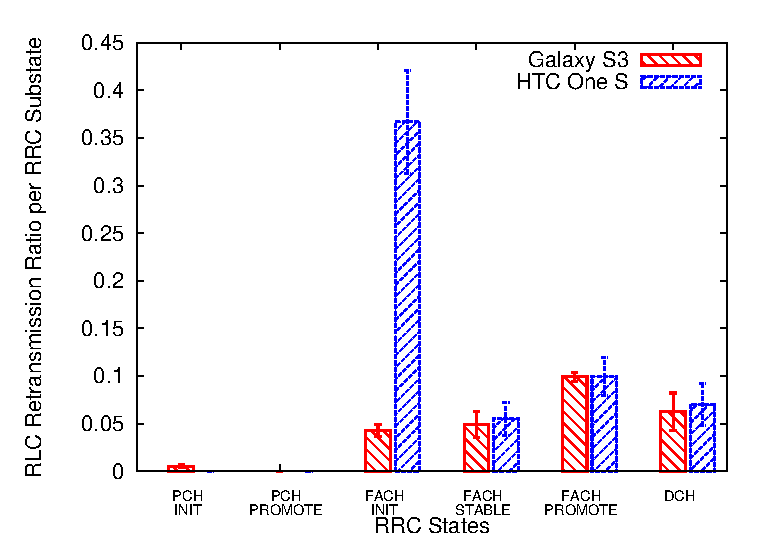
\includegraphics[width=0.5\textwidth]{figs_nonanony/rlc_retx_udp.eps}
\ncaption{The significant RLC retransmission ratio over the stable FACH state and FACH promotion state is consistent with higher-layer measurements and suggests that FACH\_{}INIT has a significant impact on the FACH transition delay.}
\label{fig:RLC.Loss.Per.RRC.UDPTrace}
\end{figure}

%TCP Trace Analysis
We also examined performance in TCP. A TCP \textit{retransmission timeout} (RTO) can cause a RTT delay as the congestion window size decreases and the device falls back to the slow start phase~\cite{tcp.rto}. We use our mapping algorithm to correlate TCP retransmission behavior with RLC retransmissions. We found that the current RLC protocol responds sluggishly to the duplicate ACKs that signal that a PDU has been lost (see Figure~\ref{fig:RLC.Dup.Ack}). This leads to a TCP RTO which introduces more latency in the transport layer.  

According to the 3GPP RLC specification, the sender only retransmits the PDU once it receives a STATUS LIST (i.e., non-acknowledged) control PDU from the receiver, ignoring duplicate ACKs~\cite{spec-3G-RLC}. These duplicate ACKs are strong hints for PDU losses. If the lost RLC PDUs were to be transmitted after 0.5s rather than 2.8s, then the TCP RTO could be avoided, reducing latency by more than 2.3s. We propose a RLC \textit{Fast Re-Tx} mechanism, where unacknowledged PDUs are retransmitted once three duplicate RLC PDU ACKs are received by the sender. The resulting faster reaction to lost signals would reduce both RLC latency and latency in the transport layer. We evaluate this mechanism in \S\ref{sec:eval}

%The TCP retransmission timeout (RTO) could cause apparent round trip delay due to congestion window drop by half and restarting the data transmission from the slow start phase~\cite{tcp.rto}. From the \emph{QxDM\_{}Trace}, we correlate the TCP retransmission behavior with the RLC retransmission through our mapping algorithm. By capturing the root cause of the TCP RTO, we found that current RLC protocol has a sluggish response to the PDU lost sigals -- the duplicate ACKs, in Figure~\ref{fig:RLC.Dup.Ack}. The delayed RLC retransmission PDUs leads TCP RTO, which further introduces latency in the transport layer. In 3GPP RLC specification, the sender only retransmits the PDU once it receives the STATUS LIST (or non-acknowledged) control PDU from the receiver, but ignores to duplicate ACKs, which is a strong hint for PDU loss~\cite{spec-3G-RLC}. If we could bring the group of retransmitted RLC PDUs from 2.8 s to 0.5 s, then we could avoid TCP RTO, reducing the latency more than 2.3 s. Therefore, we propose a RLC \textit{Fast Re-Tx} mechanism, which will retransmit the unacknowledged PDUs once the sender receives three duplicate RLC PDU ACKs. The faster reaction to loss signals could reduce RLC layer latency and further reduce the latency in transport layer.

% explain the root cause of the longer delay analysis
\begin{figure}[t!]
\centering
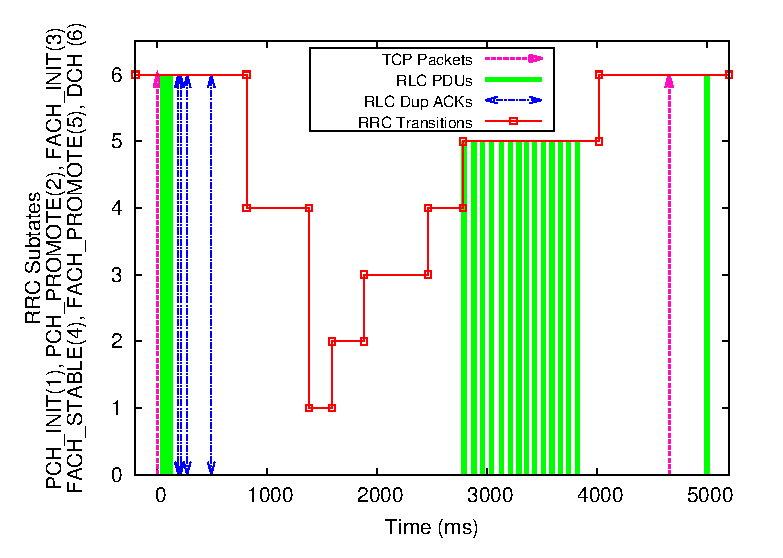
\includegraphics[width=0.5\textwidth]{figs/rlc_dup_ack.eps}
%\ncaption{Two Latency Causes: short DCH demotion timer and lagging response to the PDU lost signal}
\ncaption{TCP RTO is caused by delays in RLC PDU retransmission. Duplicate ACKs suggest a PDU has been lost. By responding to this probable loss in a timely manner, RLC transmission latency can be reduced and sometimes TCP RTOs can even be avoided.}
\label{fig:RLC.Dup.Ack}
\end{figure}

% UDP loss analysis
%\subsubsection{Root Cause of Packet Loss}\label{sec:udp.loss.analysis}
Finally, we examine UDP losses in each RRC state and identify root causes of these losses.  We label each packet with a unique ``sequence number" to map UDP packets sent from the client to the server-side tcpdump trace --- a loss occurs when a packet never appears at the server.  We consider the RRC state or RLC-layer transient state associated with each packet to be the state when the packet is sent, as defined in Table~\ref{tab:terminology}.  Packet loss ratios are the ratios between the number of packets lost from each state and those sent.  As can be seen in Figure~\ref{fig:udp.loss}, these losses are highly device-dependent as well, with \Paperonly{the M2 device} \TReport{the HTC device} having a higher loss ratio in DCH and FACH, and the \Paperonly{M1}\TReport{Samsung} device being more lossy in PCH.  As devices perform most transmissions in DCH and FACH, the \TReport{Samsung}\Paperonly{M1} device is less lossy overall.

%UDP protocol doesn't guarantee the data package delivery, because the sender doesn't receive feedback from the receiver. We are interested in understanding the UDP loss behaviors over each RRC state, and also identify the root cause of UDP packet loss. As we instrument a unique "sequence number" for every UDP packet in \emph{QxDM\_{}TRACE}, we are able to apply the one-to-one mapping of UDP packet from client side \emph{QxDM\_{}TRACE} to the server side tcpdump trace. Each packet loss is considered as an packet appeared on the client side, but not on the server side. The RRC state of a packet means the state when it was transmitted. The packet loss ratio per RRC state is calculated as the number of packets get lost over that state divided by the total number of packets over that state. In Figure~\ref{fig:udp.loss}, the loss ratio really depends on the devices. HTC One S has a higher loss ratio over, DCH, and FACH state. While Samsung Galaxy S3 is more lossy over the PCH state. As the device is generally stay in DCH and FACH state, the Galaxy S3 will be less loss than the HTC device.

% UDP Loss Ratio plot
\begin{figure}[t!]
\centering
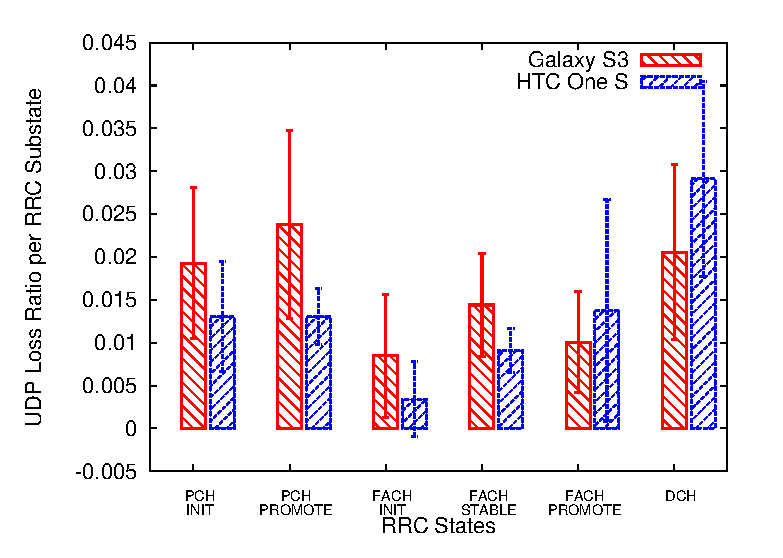
\includegraphics[width=0.5\textwidth]{figs_nonanony/udp_loss.eps}
\ncaption{UDP loss dependence on the device and on RRC transition states}
\label{fig:udp.loss}
\vspace{1ex}
\end{figure}

To identify the root cause of these UDP losses, we use the cross-layer mapping algorithm to understand RLC-layer transient state behavior.  We wish to understand if the UDP packets are getting lost over the OTA link or the wired channel as defined in \S\ref{sec:background}. Since QxDM only captures the data transmission in UTRAN, SDU losses not found in QxDM traces are lost over the wired channel. According to the 3GPP specification~\cite{spec-3G-RLC}, RLC PDUs are lost between the handset and the Node-B due either to senders retransmitting the PDUs more times than a pre-defined limit or due to the sender being reset by the receiver.  After mapping each UDP PDU to the corresponding RLC PDU, we check if the sender received a reset control PDU from the receiver or if the number of retransmitted PDUs exceeds a predefined limit.  If neither case applies, we know that the the UDP packet was lost over the internet.  Most UDP packets are lost over the wired channel, as can be seen in Figure~\ref{tab:udp.loss.root.cause}. This is due to the RLC layer ARQ (Automatic Repeat reQuest) mechanism that limits losses in the RLC layer.

%The UMTS network consists of the mobile devices, the \textit{UMTS Terrestrial Radio Access Network} (UTRAN), and the \textit{Core Network} (CN)

%To identify the root cause of the UDP loss, we apply the cross-layer mapping algorithm, and analyze the RLC layer behaviors. We are interested in whether the UDP packets get lost in the cellular network or in the internet. Based on 3GPP specificaiton~\cite{spec-3G-RLC}, RLC PDUs will be lost in between the handset and the Node-B, because either the sender retransmit the PDU more than a pre-defined limit or the sender was reset by the receiver. After map each UDP packet with a corresponding RLC PDUs, we will check whether the sender received a reset control PDU from the receiver, or the number of retransmitted PDU exceeding the pre-defined limit. The rest of the cases would count as the UDP lost over the internet. In Figure~\ref{fig:udp.loss.root.cause}, most of the UDP packets are lost over the internet, which is primarily because the RLC layer ARQ (Automatic Repeat reQuest) mechanism in the RLC layer. 

% UDP Loss Root Cause
%\begin{figure}[t!]
%\centering
%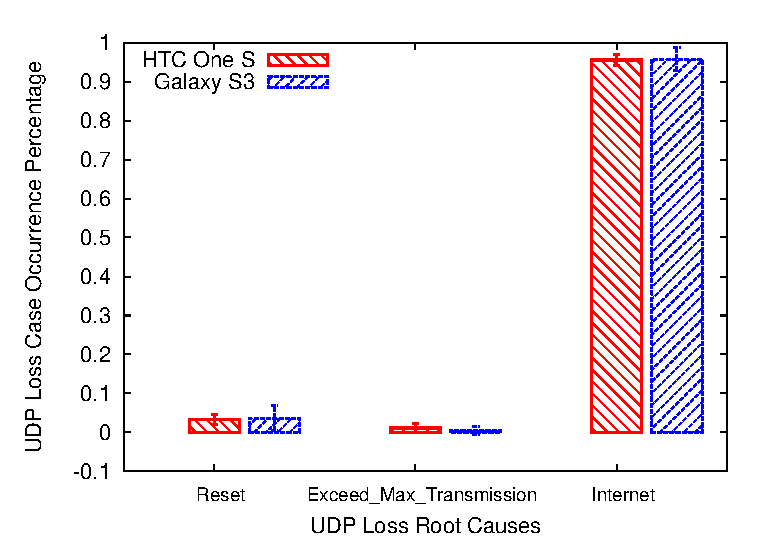
\includegraphics[width=0.5\textwidth]{figs/udp_loss_root_cause.eps}
%\ncaption{The major loss cause of UDP packets comes from internet, but not in the cellular network}
%\label{fig:udp.loss.root.cause}
%\end{figure}

\begin{table}\small
\begin{tabularx}{0.5\textwidth}{|X|X|X|X|}
	\hline
	& \multicolumn{2}{|c|}{\textbf{OTA (\%)}} & \multirow{2}{*}{\textbf{\vbox{Wired (\%)}}} \\ \cline{2-3}
	& \textbf{Reset} & \textbf{Exceed Limit} & \\
	\hline\hline
	\Paperonly{Device M1}\TReport{Samsung SIII} & 3.67$\pm$3.14 & 0.57$\pm$1.01 & 95.77$\pm$3.01 \\
	\hline
	\Paperonly{Device M2}\TReport{HTC One} & 3.32$\pm$1.31 & 1.17$\pm$1.16 & 95.56$\pm$1.37 \\
	\hline
\end{tabularx}
\ncaption{Most UDP packet losses happen in the wired network, not the OTA (or wireless) channel.}
\label{tab:udp.loss.root.cause}
\end{table}

\subsection{Public Deployment of the Inference Tool}\label{sec:largescalestudy}

To get a broader and more representative set of data, we integrated the coarse-grained RTT measurement functionality into Mobiperf~\cite{mobiperf}, an existing network performance measurement application. 
We did not collect data on the impact of RRC state on higher-level protocols, however.


130 devices on 41 carriers in 25 countries have installed the test, based on hashed phone identifiers (to preserve user anonymity). However, we only have complete data on 27 devices, covering 9 countries, 16 carriers and 20 distinct device models from 6 manufacturers.  

%\begin{TReports}
% However, there are two subsets of this data set we exclude.  First, a number of devices (48 in total) never completed sufficient tests.  
%\end{TReports}
We excluded devices with less than three tests run in order to ensure we could effectively filter noise.
\begin{TReports} 
Second, a number of devices never uploaded accurate data on the network technology used --- either because they never updated from the original application version that did not collect this data, or because their device always returns the value "UNKNOWN". We exclude these devices from any findings that require knowing the specific network technology.   We therefore focus on 27 devices with complete data in this section --- these cover 9 countries, 16 carriers and 20 distinct device models from six manufacturers.  

\end{TReports}
%such as the US, Germany, the UAE, Indonesia and China.  Phone identifiers were hashed to preserve user anonymity.  Because of the incomplete data provided by devices in the public test, N devices never uploaded sufficient data to perform the RRC inference task.  N devices had their RRC model flagged as ``anomalous" and after a manual inspection were disregarded due to having insufficient data.
%TODO fill in numbers

In this section, as we are observing higher-level behavior, we do not discuss the transient states directly.  Instead, we refer to the behavior caused by delays during transient states, resulting in UDP-layer delays when sending packets during the transient states associated with a state demotion, as FACH\_{}TRANSITION or LTE\_{}TRANSITION.  The former refers to delays when demoting to FACH, and the latter to delays when demoting to RRC\_{}IDLE.

First, we examine the inferred RRC states for the devices for which data has been collected and examine how these states vary across carriers.  For LTE, we have data from two carriers, both within the U.S.  Both have $T_{Tail}$ timers of 10 seconds.  Some devices exhibited a spike in latency when transitioning between states. There appears to be some device dependency for this effect under LTE as well. A comparison of the latencies and packet losses for two different devices using the same carrier and the same RRC state transition timers can be seen in Figure~\ref{fig:device_compare}. 

The UMTS timers are more varied, and we have more data on a wider range of carriers than for LTE.  The timers are summarized in Figure~\ref{fig:timer_cdf}. Each distinct RRC state machine for a carrier is counted only once regardless of the number of devices collecting data.  Timers are generally closer to 3 seconds when FACH is used and 7 seconds when it is not.  We do not in general have enough data to compare carriers across devices or locations, but when we do, state machine timers are consistent within one second. However, we found that one carrier which uses two different UMTS versions in two different locations has two different sets of timers.  We found that  devices usually enter FACH both during demotion and promotion, or not at all, with one exception where the device promotes directly to DCH but enters FACH during demotion.  


Substantial delays when demoting from DCH to FACH were common. It is less immediately clear that this is device-dependent behavior, though, for two reasons.  First, there are more carriers in this dataset but few devices per carrier, so comparing different devices with the same carrier is often not possible. We did observe for one carrier\TReport{, Verizon,} that not all devices exhibited this behavior, however.  Secondly, there were two cases where, for a specific model of phone, some devices exhibited this behavior and some did not. After some investigation, it seems that different chipsets are used in different markets for the same model of phone, which might explain this discrepancy.  We also determined that several different chipsets from several different manufacturers exhibit this behavior, so the problem is not due to a single poor implementation. However, without more information about each device we cannot be confident in our claim that this is entirely device-specific behavior.

%As can be seen in Figure~\ref{fig:timer_cdf}, certain timers are particularly common. There are a limited number of different RRC state machines that seem to be implemented in practice, even accross very different carriers, and this is especially true for LTE.  Timers of 6-7 seconds for LTE seem to be most common, although in the US timers of 10 seconds were frequently observed. For 3G, there is far more variation, but usually devices fall back to FACH within 2.5 to 4.5 seconds.  FACH can last from 3-5 seconds, with lower values being far more common.


%For most carriers, we have only a small number of devices per carrier, and so it is difficult to determine if the RRC state machine for a specific carrier varies by device or location.  However, for several major US carriers we had a number of different users accross the country.  For example, for AT\&T, we collected data from users in Michigan, California, Pensylvania, and Florida.  The inferred timers for each network technology are almost always consistent accross these geographic regions, within half a second.  The one exception is Verizon ---  we observed two different LTE timers in two different geographic locations with the same model of phone.  

%UMTS allows variation both in the timers between states and in the states available.  As was shown in previous work, some carriers will skip the FACH state either when promoting or demoting\cite{3g_rrc}. We found five distinct 3G RRC state machines that always pass through FACH in both directions, and six that do not enter FACH when promoting from IDLE.  Four additional carriers had the FACH state entirely obscured by the FACH\_{}TRANSITION effect. In those cases it is unclear if FACH is ever entered, but users would not benefit from FACH. Additionally, ten devices did not upload carrier information. Eight entered FACH in both directions, and two did not enter FACH during state promotion.  Most carriers within the US have state machines that enter FACH in both directions, aside from Verizon which exhibited both patterns.  No other RRC state machine patterns were observed.

%, specifically, allows more variation in how it is implemented. As was shown in previous work, some carriers will, upon recieving a packet in IDLE, go directly to DCH regardless of the size of the packet, whereas others might first pass through FACH~\cite{3g_rrc}.  In our survey of carriers, we found five distinct RRC state machines that always pass through FACH whether promoting or demoting, and six that do not enter FACH when promoting from IDLE.  There were four additional RRC state machines where data was sufficiently noisy that a significant number of measurements taken were ambiguous; three of these had the majority of their measurements consistent with entering FACH in both scenarios.  Additionally, eight devices which lacked carrier information entered FACH in both directions, and two did not enter FACH when promoting.

%Single-directional FACH state machines were most common outside of the US; additionally, Verizon exhibited both patterns on different devices.  We did not observe any other RRC state machine patterns. 




\begin{figure}[t!]
\begin{center}
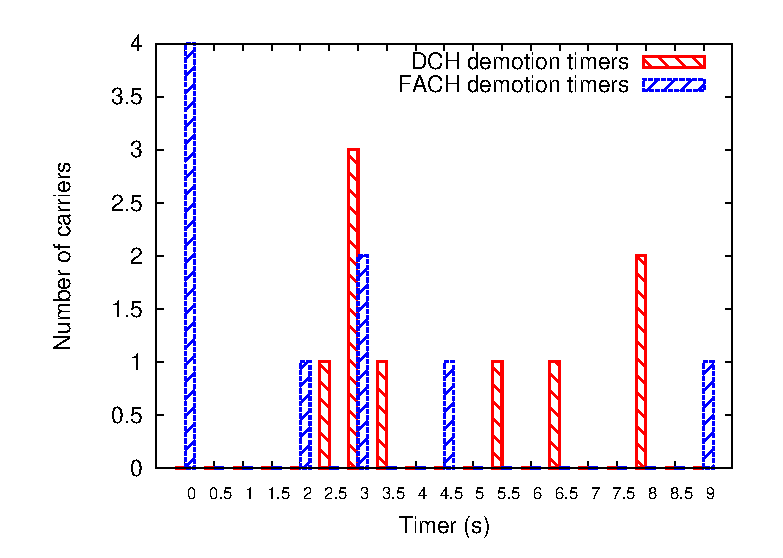
\includegraphics[width=0.45\textwidth]{figs/timer_cdf.eps}
\end{center}
\ncaption{Distribution of RRC 3G timers, for nine UMTS RRC state machines. Note cluster around 2-3.5s.}
\label{fig:timer_cdf}
\end{figure}

\begin{figure}[t!]
\begin{center}
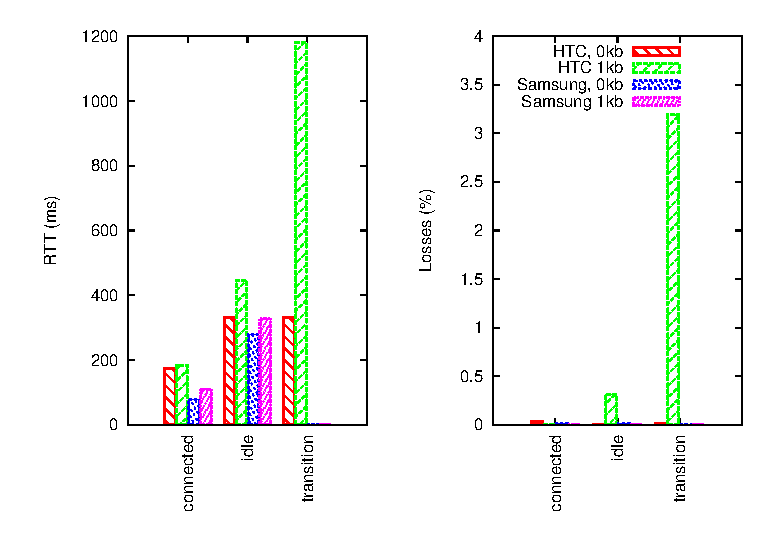
\includegraphics[width=0.5\textwidth]{figs/device_compare.eps}
\end{center}
\ncaption{RTTs and loss rates for two device models on the same LTE network, based on 39 tests for \Paperonly{M1} \TReport{the Samsung SIII} and 94 for \Paperonly{M2}\TReport{ the HTC One}.  Note that only the \TReport{HTC} device \Paperonly{M2} exhibits an additional delay around state demotion. The ``Transition" data is during a period of high latency when sending data around a demotion to RRC\_{}IDLE.}
%\ncaption{RTTs and loss rates for an HTC One and Samsung S3 device on the same LTE network.  Note that only the HTC device exhibits an additional delay around state demotion.}
\label{fig:device_compare}
\end{figure}
We also examined the performance characteristics associated with different RRC states. As most of our data was for LTE or UMTS, we focus on these two technologies. For UMTS, we collected data from 12 devices. Between 16 and 143 tests were run per device (with an average of 70 tests run). We excluded a large number of devices with less than three tests each --- the distribution of measurements per device is very irregular. For LTE, we used 9 devices with an average of 34 tests each, ranging from 4 to 110 tests.

We first  examined the average promotion delays associated with different RRC states, shown in Figure~\ref{fig:all_carrier_rrc_delays}. These are calculated based on the difference in RTT between the highest-power, lowest-latency state and every other RRC state. We see that the pattern we observed for the \Paperonly{Carrier C1}\TReport{controlled T-mobile} dataset holds here as well. Furthermore, LTE generally performs better than 3G.  It can also be seen here that latencies when transitioning between DCH and FACH are quite substantial, and often higher than in PCH.

\begin{figure}[t!]
\begin{center}
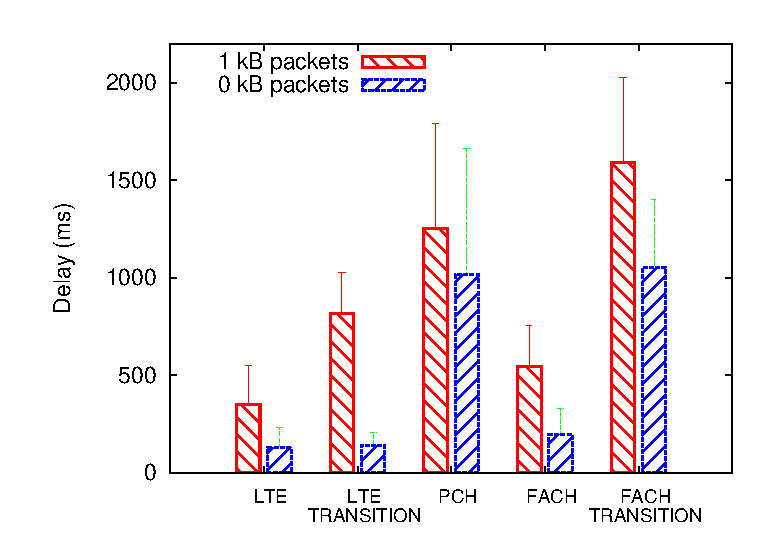
\includegraphics[width=0.45\textwidth]{figs/all_carrier_rrc_delays.eps}
\end{center}
\ncaption{Promotion delays for each state for all carriers surveyed, calculated by subtracting the RTT in the highest-power state from the RTTs in states where promotions are required.  The anomalous behavior FACH\_{}TRANSITION and LTE\_{}TRANSITION, when it occurs, results in significant delays.}
\label{fig:all_carrier_rrc_delays}
\end{figure}

We also examined trends in packet loss in different RRC states for these carriers, as shown in Figure~\ref{fig:loss_compare}, again comparing 3G and LTE.  Unsurprisingly, losses were generally low in high-power states (DCH or RRC\_{}CONNECTED) and are high in low-power states. This is especially true in LTE.  Although in LTE the state transition delay results in less of an increase in latency, it does appear to result in relatively high packet loss.  Furthermore, FACH does not perform well in terms of packet loss either. 

%\mycomment{Why are losses higher for smaller packets? Is this expected behavior?}

%\mycomment{If time permits perform this analyis for our T-Mobile data set, however due to the database problems this sort of analysis may be more time-consuming to do (as I'm currently parsing a giant dump of the database contents)}



%\mycomment{I suspect this occurs more when we get the bad FACH behavior, would be good to verify}

\begin{figure}[t!]
\begin{center}
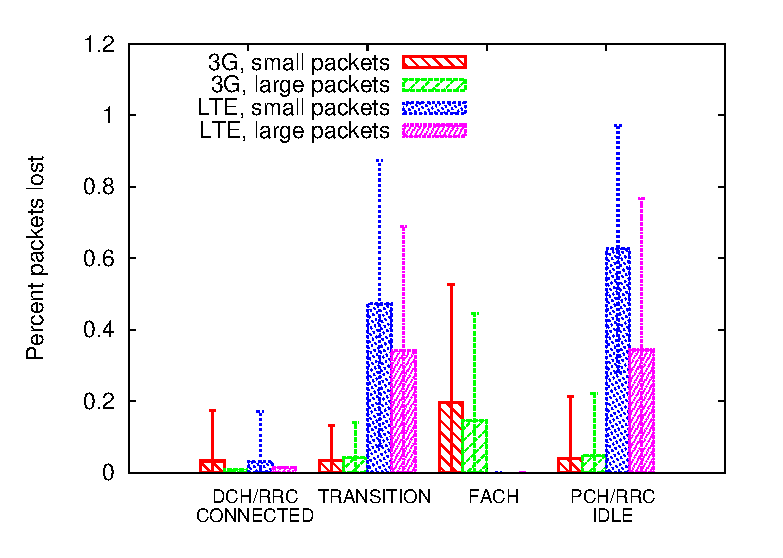
\includegraphics[width=0.45\textwidth]{figs/loss_compare.eps}
\end{center}
\ncaption{Packets lost per state as a percent. Note high losses during transition and RRC\_{}IDLE for LTE.} 
\label{fig:loss_compare}
\end{figure}

Overall, it can be seen that the phenomena we have observed in our controlled experiments on \Paperonly{Carrier C1}\TReport{T-Mobile} devices are of more universal relevance, and more generally that our client-based inference methodology is an effective way to understand trends in RRC state implementations and performance more broadly.   Our inference technique has additionally allowed us to measure the performance characteristics of networks on consumer devices, without requiring any expert knowledge to collect the needed data.



%\mycomment{Tmobile timers consistent.  Only variation is FACH noise for UMTS.  EDGE: timer 1.5s, no FACH-like state.  HSDPA: only one data point, timer 3s, no FACH.  LTE: timer 2s, one data point and kind of noisy (but collecting data on a second data point).  UMTS: 2.5s timer for DCH and another 2.5 on FACH, often eaten by demotion-related delay.}



%\begin{figure}[t!]
%\begin{center}
%
\includegraphics[width=0.45\textwidth]{figs/placeholder.png}
%\end{center}
%\ncaption{Performance for each device for T-Mobile only; colour-code by geographic state - TODO - not much interesting data? lower priority}
%\label{fig:fach_demotion_delay_prevalence}
%\end{figure}

\section{Evaluation}

\subsection{RTT Estimation}
We first define the RTT in RLC layer. In the RLC protocol, the STATUS PDUs (ACK or NACK) don't generate by every received RLC PDU, but triggered either by receiving a polling request from the sender or by detecting one or more missed PDUs from its receiver buffer~\cite{spec-3G-RLC}. Since the QxDM traces are collected at the client side, we don't have the information of when the server side receive the PDU. Thus, I estimate the RTT of a RLC PDU based on the timestamp difference between the most recent sender's polling request and received ACK. Based on RLC configuration, the maximum polling request frequency is 500 ms. One of the previous mobile RTT estimation study shows the autocorrelation coefficient of two RTT measurements within 500 ms is more than 0.6~\cite{proteus}. Therefore, my estimation is still reasonable to be considered as the real RLC RTT value.

\subsection{Cost-Benefit Analysis}
In order to know whether the new proposed RLC mechanism works, I apply a cost-benefit analysis over the existing \emph{TCP\_{}Trace}. The definition of benefit and cost is straight forward. Basically, if the fast retransmitted PDUs will be transmitted in the future, then we compare the RTT if it transmitted right after the duplicate ACKs with the real RTT value in the trace. If the difference is less than 0, we call that is a benefit. In the same way, if it is greater than 0, we call it a cost. However, we want to know if the PDU is really lost over the channel, or it just gets delayed due to channel contention. That depends on whether the sender receives a ACK or NACK (a list of unreceived PDU sequence numbers). We categorize the situations into four cases -- Win, Draw\_{}Plus, Draw\_{}Minus, and Loss. If the sender will receive a NACK, and more than 50\% of the fast retransmitted PDUs will retransmit in the real trace, then we call the case "Draw\_{}Plus" as in Figure~\ref{fig:draw.plus}. Since it would brings us benefit if the fast retransmit RTT is less than the RTT in the real trace. The "Win" case is defined that if we could avoid a TCP RTO based on the "Draw\_{}Plus" in Figure~\ref{fig:win}. In that case, RLC layer benefit is the same as "Draw\_{}Plus", but I want to highlight that it could bring further latency benefit over the transport layer. "Draw\_{}Minus" occurs when less than 50\% of the fast retransmitted PDUs get really retransmitted in the real trace as in Figure~\ref{fig:draw.minus}. If the sender gets a ACK with a larger sequence number, then all the PDUs were successfully delivered to the receiver. In that case, we called the case "Loss", since all the retransmitted packets are redundant as in Figure~\ref{fig:loss}. To summarize all four cases:

\begin{itemize}
\item \textbf{Win:} A special case of Draw\_{}Plus with extra benefit of avoid TCP RTO.
\item \textbf{Draw\_{}Plus:} More than half of the fast retransmitted packets really retransmitted in the real trace.
\item \textbf{Draw\_{}Minus:} Less than half of the fast retransmitted packets really retransmitted in the real trace.
\item \textbf{Loss:} None of the fast retransmitted packets retransmitted in the real trace.
\end{itemize}

% Four cases
\begin{figure}[h!]
\centering
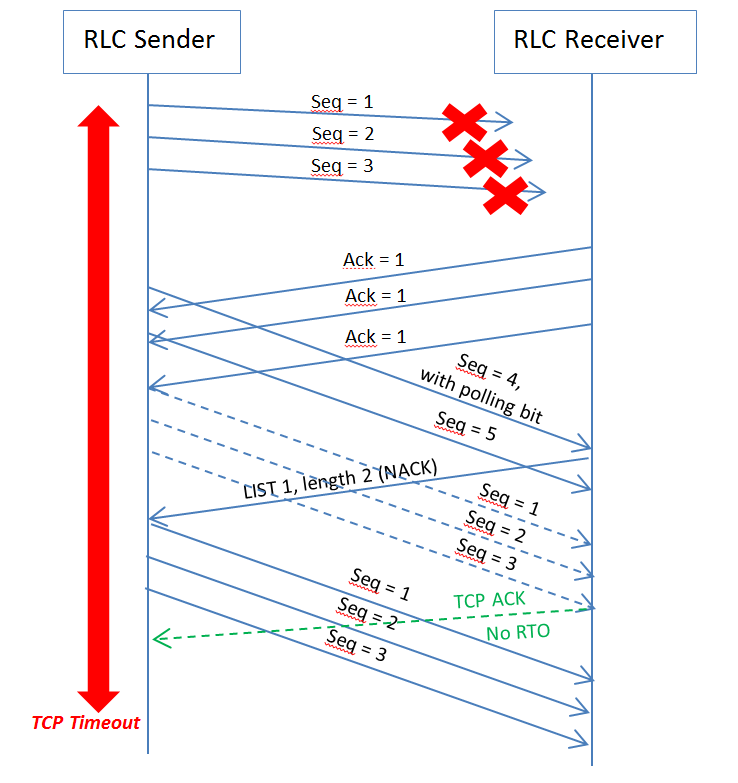
\includegraphics[width=0.45\textwidth]{figs/Win.png}
\caption{Win: RLC Fast Re-Tx avoid a TCP RTO}
\label{fig:win}
\end{figure}

\begin{figure}[h!]
\centering
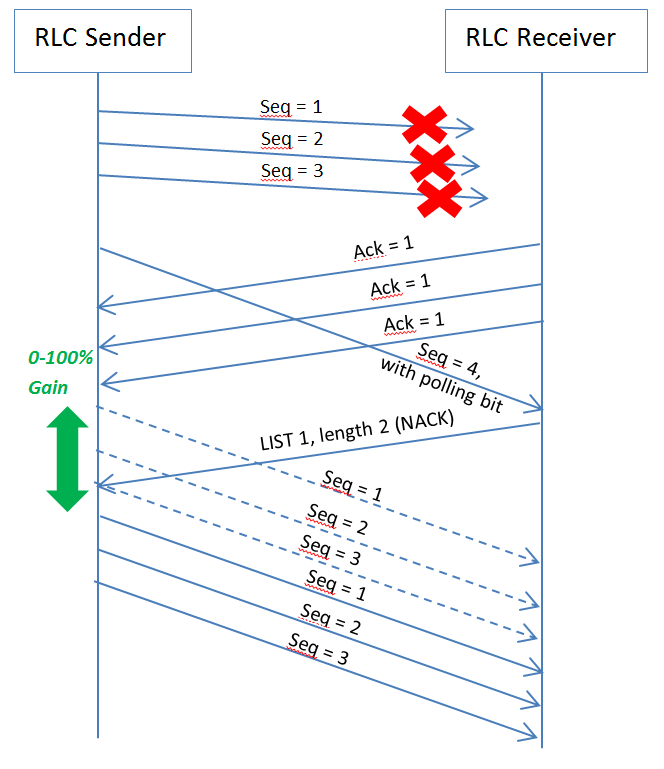
\includegraphics[width=0.45\textwidth]{figs/Draw_plus.png}
\caption{Draw Plus: the predication accuracy is more than 50\%}
\label{fig:draw.plus}
\end{figure}

\begin{figure}[h!]
\centering
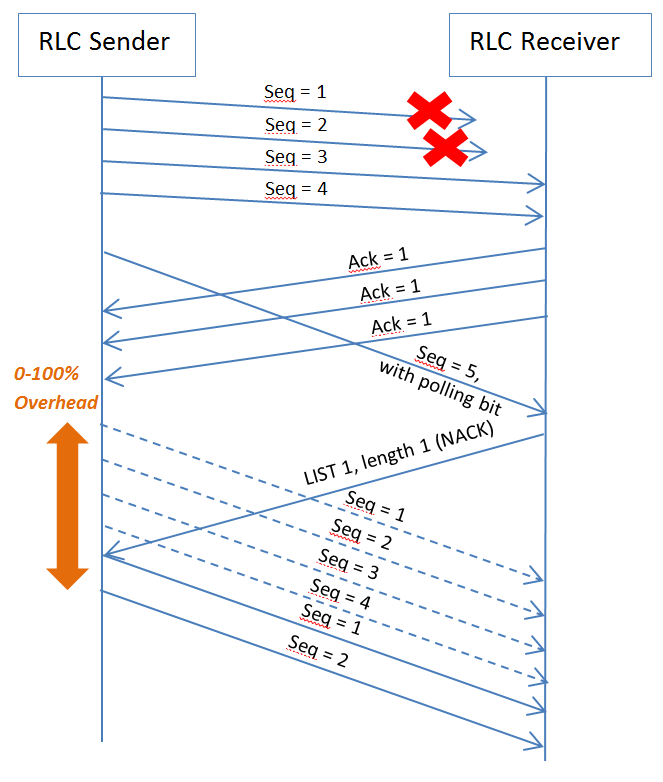
\includegraphics[width=0.45\textwidth]{figs/Draw.png}
\caption{Draw Minus: the predication accuracy is less than 50\%}
\label{fig:draw.minus}
\end{figure}

\begin{figure}[h!]
\centering
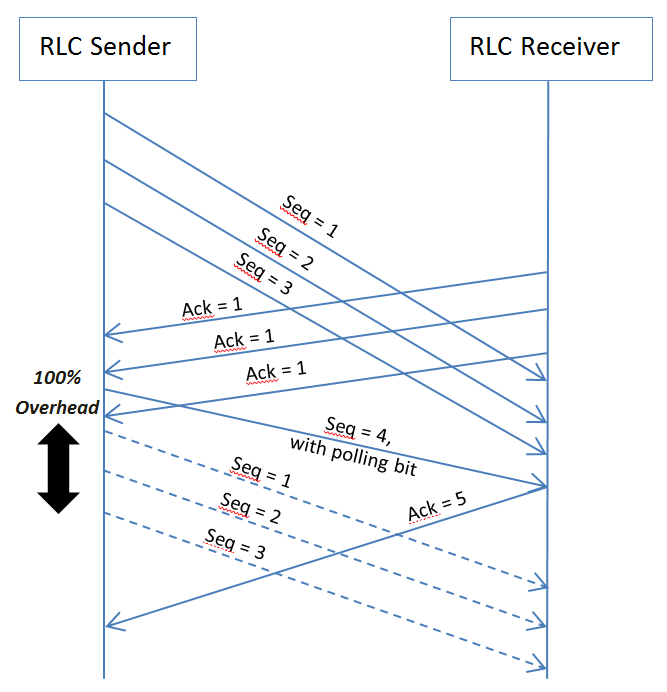
\includegraphics[width=0.45\textwidth]{figs/Loss.png}
\caption{Loss: all predications fail}
\label{fig:loss}
\end{figure}

As we can see from Table~\ref{tab:rlc.fast.sim}, around 75\% of the time we will have benefit on RLC latency reduction if we count the "Win" and "Draw\_{}Plus". The overall RLC delay could be reduced by \textit{2.66\%} over all the RRC state based on trace simulation analysis. If we break down the cost-benefit over different RRC states, the RLC RTT latency could reduce by up to \textit{35.69\%} over initial FACH state or FACH promotion transitions. Therefore, we could have a large latency benefit over the initial period of data transmission.


% Cost-Benefit Table
\begin{table}[h!]
\begin{tabularx}{0.48\textwidth}{ | c | X |}
	\hline
	\textbf{Case Name} & \textbf{Percentage of Occurrence (\%)} \\
	\hline\hline
  	Win & 10.32$\pm$1.89 \\
  	\hline
  	Draw\_{Plus}* & 64.68$\pm$8.32 \\
  	\hline
  	Draw\_{Minus} & 20.63$\pm$3.45 \\
  	\hline
  	Loss & 4.25$\pm$0.06 \\
  	\hline
\end{tabularx}
* The Draw\_{Plus} case excludes the percentage of Win
\caption{The RLC Fast Re-Tx Cost-Benefit Table}
\label{tab:rlc.fast.sim}
\end{table}


\label{sec:eval}


\section{Related Work}

Previous work has been done on measuring the power and performance characteristics of 3G RRC state machines~\cite{3g_rrc} as well as 4G LTE networks~\cite{4g_rrc, drx_analysis} in controlled environments, as well as specific features of those networks such as DRX~\cite{drx}.  Work has also been done on exploring the implications on application performance of RRC state and inadequacies in how mobile applications deal with RRC state~\cite{aro}.  

We expand upon this work by implementing an RRC inference method that can be integrated into a measurement tool intended for non-experts. It can automatically infer the RRC state machine of any network type, allowing anomalous or unexpected behavior to be measured, unlike previous work that assumes that devices follow the ideal behavior defined in the specification. We also focus on \emph{transient states} we observe at the RLC level related to promotions and demotions, and their impact on higher-layer performance.   Work by Souders~\cite{souder} measures RRC state machines on client devices, but being a browser-based solution it is not able to account for background activity on the phone or varying network types, measure performance data as accurately as an application can, or observe RLC-level behavior.

Other work has been done on optimizing the use of the cellular network based on 3G or 4G specific phenomena. RadioJockey~\cite{radiojockey} investigates how to effectively trigger fast dormancy based on network traffic patterns, and TailEnder~\cite{tailender} and work by Deng et al.~\cite{trafficaware} propose a method of scheduling data transfers to minimize energy consumption without impacting user-perceived performance.


Related to our RLC fast retransmission proposal, a previous study provides cross comparison analysis over the TCP and RLC protocols, and optimizes the default protocol parameters~\cite{opt.tcp.rlc}. Their primary goal is to improve the performance behavior by introducing TCP congestion control mechanism into the RLC layer. However, their traces are purely generated from simulation software, whereas we use real traffic traces. 

More generally, work has been done to measure performance characteristics of cellular networks and networks on mobile devices. The Livelab project~\cite{livelab} also makes use of users running a measurement app on their phones. A wide range of findings on how users interact with mobile devices have been published, including  measuring web usage in the wild~\cite{livelab-webusage}. Work by Halepovic et al.,~\cite{http_measure} presents a method of passively measuring HTTP transaction latency. Work by Gember et al.,~\cite{incontext} determines how to accurately measure user-perceived performance on user devices. JamLogger~\cite{jamlogger} is an ongoing project to collect general performance and user activity on mobile devices. Our work is complementary to these studies.


%Beyond deployments and testbeds: Experiences with public usage on vehicular WiFi hotspots

%Aditya Akella 	University of Wisconsin
%    Obtaining Representative Measurements of Cellular Network Performance 
%    Explores other factors (network traffic, location etc) that effects measurements
%    Identify that a wide range of factors can affect measurements - we care about relative values
%
%Aruna Balasubramanian 	UW
%     Energy Consumption in Mobile Phones: A Measurement Study and Implications for Network Applications 
%        Tail energy: TailEnder: schedule to avoid tail times

%Joel Sommers 	Colgate University
%    Are Smaller Packets Less Likely to be Lost?:
%    for cellular

% Jamlogger: collects a variety of system statistics periodically in the background; does not have the same challenges as a system looking for specific data, both in measurement cost and in scheduling.  Mobiperf also is not concerned with covering location in the same way and does not have the same challenges.

% LiveLab: Measuring Wireless Networks and Smartphone Users in the Field
% MEasure general real-world smartphone usage and wireless networks. Also uses interrupt-based logging, periodic logging, and collecting when idle.  Hitch-hike onto existing wakeups.  Vary frequency based on context.  More general measurements.  They don't describe power in detail, though - it's a short pape

\section{conclusion}
In this paper, we have presented new techniques for detecting and analyzing RRC state behavior and performance.  We have created a tool suitable for automatically inferring RRC state machines on end-user devices without requiring expert knowledge to run. We have demonstrated that it is effective in understanding RRC state implementations and their performance characteristics and how these vary by carrier and device model.  We have also shown that this tool is effective at uncovering previously unknown anomalous behavior, in particular that related to state transitions.  Finally, we used RLC-level analysis and a novel cross-layer analysis technique to uncover some underlying causes of these unexpected phenomena, and show how they relate to RLC-layer \emph{transient states}.  We proposed RLC \emph{Fast Re-Tx} mechanism that reduces the RLC latency up to 35.69\% during FACH\_{}TRANSITION.

%\newpage \clearpage\setcounter{page}{1}
\bibliographystyle{abbrv}
\bibliography{robustnet}  % sigproc.bib is the name of the Bibliography in this case
\end{document}

